\documentclass[11pt,letterpaper]{article}
\usepackage[T1]{fontenc}
\usepackage[utf8]{inputenc}
\usepackage{lmodern,microtype}
\usepackage[margin=1in,headheight=14pt]{geometry}
\usepackage{amsmath,amssymb,amsthm,mathtools}
\usepackage{booktabs,array,longtable,tabularx}
\usepackage{enumitem,graphicx,xcolor,fancyhdr}
\usepackage{listings}
\usepackage{xurl}
\usepackage[numbers,sort&compress]{natbib}
\usepackage[colorlinks=true,linkcolor=blue!45!black,citecolor=blue!45!black,urlcolor=blue!50!black,breaklinks=true]{hyperref}
\usepackage{bookmark}
\definecolor{ink}{HTML}{19354A}
\definecolor{pale}{HTML}{F3F6F8}
\hypersetup{pdftitle={Toward Quasi-Polynomial Unknot Recognition: Presentation Complexity, Early Certificates, and Streaming Responses},pdfauthor={Research continuation for the ProveIt project},pdfsubject={Exact parameterized algorithms, audited implementation, and research agenda}}
\setlength{\parindent}{1.2em}
\setlength{\parskip}{0.2em}
\setlength{\emergencystretch}{1.8em}
\setcounter{tocdepth}{2}
\setlist{itemsep=0.3em,topsep=0.45em}
\newtheorem{theorem}{Theorem}[section]
\newtheorem{proposition}[theorem]{Proposition}
\newtheorem{lemma}[theorem]{Lemma}
\newtheorem{corollary}[theorem]{Corollary}
\theoremstyle{definition}
\newtheorem{definition}[theorem]{Definition}
\newtheorem{remark}[theorem]{Remark}
\newcommand{\F}{\mathbb F}
\newcommand{\poly}{\operatorname{poly}}
\newcommand{\rank}{\operatorname{rank}}
\newcommand{\Kh}{\operatorname{Kh}}
\newcommand{\basecommit}{\texttt{1be2abc8cc743c1a3b5cb7fdfeb650697f8e2d5b}}
\newcolumntype{Y}{>{\raggedright\arraybackslash}X}
\lstset{basicstyle=\ttfamily\small,backgroundcolor=\color{pale},frame=single,rulecolor=\color{black!15},breaklines=true,columns=fullflexible,keepspaces=true,showstringspaces=false,xleftmargin=0.4em,xrightmargin=0.4em,aboveskip=0.7em,belowskip=0.7em}
\pagestyle{fancy}
\fancyhf{}
\fancyhead[L]{\small\color{ink}ProveIt: unknot recognition}
\fancyhead[R]{\small Research continuation, October 2026}
\fancyfoot[C]{\thepage}
\renewcommand{\headrulewidth}{0.3pt}

\begin{document}
\hypersetup{pageanchor=false}
\begin{titlepage}
\vspace*{0.25in}
{\Large\sffamily\color{ink}PROVEIT\quad /\quad TOPOLOGY\par}
\vspace{0.35in}
{\LARGE\bfseries Toward Quasi-Polynomial\\[0.12em] Unknot Recognition\par}
\vspace{0.22in}
{\Large Presentation complexity, early first-jet certificates,\\[0.12em]
and streaming boundary responses\par}
\vspace{0.45in}
{\large Research continuation prepared for Vladimir Reshetnikov\par}
\vspace{0.08in}
{8 October 2026\par}
\vspace{0.45in}
\begin{abstract}
We develop three exact improvements to the ProveIt unknot-recognition
program, separating complete parameterized decision theorems from optional
implementation experiments. First, a presentation with $r$ generators and
total explicit relator length $N$ yields deterministic recognition in
$\poly(N+r)(2+N/r)^{O(r)}$ bit operations, after verified provenance is
included. A straight-line word presentation gives a constant-degree
formulation with cost $\poly(S+r+s)2^{O(r+s)}$; a cut through its word
circuit gives $\poly(S+r+s)(d+2)^{O(r+t)}$. The proofs account for dense
polynomial construction, coefficient height, inverse letters, conjugate
meridians, and degenerate gauge choices.

Second, two binary matrix ranks compute a one-matching complex's scalar
survivors and first-jet closure multiplier before cobordism elimination.
A rigidity theorem at multiplier one proves equality of total Khovanov
rank under every classical link continuation. A separate flat-origin
constraint explains why the stronger algebraic interval compression is
absent from genuine minimal complexes in the tested corpus.

Third, a reverse filtration of cut faces compiles all suffix determinant
responses in $O(n(W+1)^2)$ field operations, retaining singular interior
directions and handling characteristic two. Controlled experiments show
substantial response-setup improvements, mixed early-observer performance,
and useful small-instance exact algebraic decisions. All inconclusive
solver outcomes and unfavorable timings are retained.

The work supplies proved sufficient quasi-polynomial regimes and explicit
obstructions to universal whole-group compression. It does not establish
a quasi-polynomial bound for the full maintained recognizer. We conclude
with a prioritized research program, concrete proof obligations, a patch
against a pinned repository revision, and reproducibility artifacts.
\end{abstract}
\vfill
{\small Source baseline: \basecommit.\\
Repository: \href{https://github.com/VladimirReshetnikov/ProveIt/tree/main/Topology/UnknotRecognition}{ProveIt / Topology / UnknotRecognition}.\\
Companion archive contains source, exact inputs, raw measurements, tests,
integration patch, and build instructions.}
\end{titlepage}
\pagenumbering{roman}
\hypersetup{pageanchor=true}
\tableofcontents
\clearpage
\pagenumbering{arabic}

\section{Scope, status, and the three costs being reduced}
\label{sec:overview}

The objective is a mathematically justified acceleration of the ProveIt
unknot-recognition algorithm, with quasi-polynomial asymptotic
complexity as the research target. The repository already contains a
substantial collection of exact structural certificates, compressed group
operations, and relative Khovanov scanners. A useful continuation must
identify which expensive operations it actually avoids and which input-size
parameters remain uncontrolled. This report develops three such improvements,
and includes the code and negative experimental results needed to evaluate
them independently.

\begin{definition}[Input and target]
The primary input is a validated spherical planar diagram of a tame knot
with $n$ crossings and one component. Crossing and edge labels have
polynomially bounded encoding length after normalization. General
quasi-polynomial time means $\exp((\log(n+2))^{O(1)})$; several sufficient
conditions in this report yield the more specific bound
$\exp(O((\log(n+2))^2))=n^{O(\log n)}$. Bounds for a supplied compressed
presentation explicitly include its description length and provenance.
\end{definition}

Three different costs occur. The first is the number of real variables and
the polynomial degree in an exact representation query. The second is
cobordism-valued elimination performed before a decision certificate becomes
visible. The third is repeatedly eliminating the same graph interior while
preparing boundary observations at successive stages. Reducing any one of
these can be useful. None alone bounds the total number of intermediate
relative-complex objects or guarantees a short geometric decomposition.

\begin{table}[htbp]
\centering\small
\begin{tabularx}{\textwidth}{@{}p{0.23\textwidth}YY@{}}
\toprule
Result & Proved guarantee & Remaining condition or limitation\\
\midrule
Explicit knot-group presentation &
$\poly(N+r)(2+N/r)^{O(r)}$ bit operations &
Construct and verify the presentation; $N$ counts explicitly written letters.\\
Word-circuit cut &
$\poly(S+r+s)(d+2)^{O(r+t)}$ bit operations &
Pay for retained gates, formal degree, dense compilation, and provenance.\\
Pre-elimination first jet &
$t=N-2\rank A$ and $\kappa=N-\rank\bigl(\begin{smallmatrix}A&0\\B&A\end{smallmatrix}\bigr)$ &
Whole one-matching summand; general multiplier needs a knot completion.\\
Multiplier-one rigidity &
One matching preserves total rank under every classical link continuation &
Preserves a decision quantity; original quantum grading is not retained.\\
All-suffix responses &
$O(n(W+1)^2)$ field operations for every suffix &
Prescribed order; query count and relative-complex growth are separate.\\
Checkpoint scan &
$\poly(n)2^{O(g+w)}$ for its actual maximum gap and frontier &
No universal polylogarithmic bound on $g+w$ is proved.\\
\bottomrule
\end{tabularx}
\caption{The theorem boundaries. Letters reused inside individual sections
are defined locally; in the presentation rows $r$ counts generators and $N$
counts relator letters, while in the first-jet row $N$ counts complex objects.}
\label{tab:results}
\end{table}

\subsection{What is established and what is still research}

The presentation theorems are exact decision theorems using established
existential real algorithms. The delivered compiler emits exact integer
polynomials, but its optional practical solver is NLSAT through Z3; the
theoretical running-time bound is not attributed to that solver. The
first-jet scanner is a complete rank-decision method when its underlying
exact computation is allowed to finish, with a bounded optional observer
and an unchanged mathematical fallback. The streaming-response module is
a subroutine with a proved arithmetic bound, and is not installed in the
default recognition pipeline.

The development is based on the pinned revision \basecommit\ of the
ProveIt repository \cite{ProveItBaseline}. Prior reports establish the
binary Jones contraction, scalar residue and radical analysis, first-jet
knot-completion multiplier, and fixed-stage boundary responses. The new
work is the quantitative presentation compilation, the placement of the
first-jet test before elimination together with its multiplier-one link
extension and flat-origin constraint, and reuse of boundary elimination
across all changing suffixes. Established ingredients receive attribution;
the fact that a combination is proved here does not establish historical
priority for every ingredient or parameterized consequence.

% Optional introduction/footnote material, status checked 8 October 2026.
% Bibliography keys are supplied in su2_sources.bib.

\paragraph{Current literature and the meaning of the target.}
The present work does not claim a new general quasipolynomial algorithm.
Lackenby's March 2021 author slides announce a running time
$2^{O((\log n)^3)}=n^{O((\log n)^2)}$ and outline a hierarchy approach
\cite{Lackenby2021Slides}. We use that source's displayed bound.
His July 2026 preprint proves a new hierarchy
algorithm for incompressibility, with unknot recognition as a consequence,
and explicitly leaves possible speed-ups to future work
\cite{Lackenby2026Hierarchies}.  It should therefore not be cited as a
completed proof of the announced quasipolynomial bound.  The present
algebraic sufficient condition targets $n^{O(\log n)}$ on a specified
residual class, under explicitly stated and verified compression hypotheses.
These are different statements.

A September 2026 preprint by Musick claims a polynomial-time procedure
for producing locally minimal bridge presentations and, consequently,
unknot recognition in $P$ \cite{Musick2026}.  Version 2 is dated
20 September 2026.  That claim has not been independently established by
this study and none of the results or code here depends on it.  Recording
its existence avoids the inaccurate claim that no polynomial-time preprint
has appeared; treating it as an unverified recent claim avoids replacing
proof checking with an abstract-level assertion.  An independent audit
would have to establish the completeness of the permitted presentation
moves and the polynomial bounds on their compressed execution, as well as
the correctness of the initial diagram conversion.

\paragraph{What the hierarchy bounds suggest.}
Lackenby's 2026 Proposition 9.1 bounds the number of main iterations by
$L(g+1)^L$, where $L$ controls hierarchy length and $g$ controls the
relevant pattern complexity.  The later sections develop efficient
hierarchy certificates and compressed cutting operations
\cite{Lackenby2026Hierarchies}.  Purely as an implication of that bound,
polynomial $g$ and $L=O(\log n)$ would yield $n^{O(\log n)}$
iterations, while $L=O((\log n)^2)$ yields
$n^{O((\log n)^2)}$.  Counting iterations alone still requires a bound
on the bit cost of each iteration and on the construction of the
surfaces used.  The 2021 slides describe polynomial genus, compressed
hierarchies, multisurfaces, and Heegaard/Cheeger-region arguments as the
components of that route \cite{Lackenby2021Slides}.  A rigorous
implementation project would need exact data formats, verified transition
rules, and complete size and bit-complexity bounds for those components.


\subsection{A stronger sufficient condition is useful even with obstructions}

For a word circuit, let $r$ count original generators, let $t$ count
retained gates, and let $d$ bound the formal degrees after cutting. The
explicit target
\[
             (r+t)\log(d+2)=O((\log n)^2)
\]
turns an informal request to ``compress the group'' into a testable theorem
statement. It must be accompanied by polynomial construction and verification
costs. Connected sums of trefoils, and a prime pretzel family, have group
rank growing linearly with crossing count. Thus this condition cannot hold
universally for presentations of the entire knot group. The same knots
have inexpensive coloring obstructions, so they do not refute a portfolio
that first removes such cases. A meaningful residual-class theorem must
state those filters and decompositions exactly.

Likewise, the first-jet scan supplies an explicit target $g+w=O(\log^2 n)$
on the executed order, including temporary crossing allocation and the
last segment. The streaming response theorem reduces the cost of observing
such an order without proving that the order exists. These formulations
make a future quasi-polynomial claim susceptible to proof checking rather
than extrapolation from favorable timings.

\section{The maintained algorithm and its unresolved size parameters}
\label{sec:baseline}

\subsection{The exact foundation}

The maintained program validates diagrams before applying inexpensive
structural tests, diagram simplification, invariant obstructions, and
optional certificate searches. It has specialized recognition routines for
several structured inputs and an exact Khovanov fallback. The group stage
supports explicit and straight-line words, with independent replay of
its existing certificate formats. Optional normal-surface calls have a
separate external-engine trust boundary. These are important existing
capabilities; this report does not reintroduce them as new results
\cite{ProveItBaseline}.

The homological fallback uses Bar-Natan's local tangle formalism and
cancellation \cite{BarNatan2005,BarNatan2007}. A crossing extends a relative
complex. Closed circles are delooped, scalar isomorphisms are cancelled,
and dot polynomials encode the remaining cobordisms. At final closure the
total characteristic-two Khovanov rank decides the unknot, using
Kronheimer--Mrowka's detection theorem and the characteristic-two reduced
splitting \cite{KM2011Kh,Shumakovitch2014}. Section~\ref{sec:first-jet-pre-schur}
states the exact rank convention used by the new decision scanner.

An invariant obstruction is logically asymmetric. A determinant or Jones
value incompatible with the unknot proves knottedness, but a compatible
value does not generally prove triviality. A verified reduction to the
empty diagram, a replayed group certificate, or a completed detecting
homology computation can certify the unknot. Resource exhaustion produces
an unresolved status. This asymmetry remains part of every new interface.

\subsection{Why width alone does not bound the scanner}

Let $w_s$ be the actual frontier at stage $s$, let $M_s$ be its number of
live objects, and let $L_s$ be the explicit length of its coefficient data.
A width bound controls the kinds of boundary matchings and the available
dot coordinates. It does not bound the multiplicity of each matching or
the number of homological copies. Even one fixed matching supports free
complexes with arbitrarily many objects. A bounded algebra dimension
therefore does not imply a bounded differential matrix.

Moreover, Gaussian elimination can temporarily construct large coefficient
compositions even when its final scalar survivor count is small. A correct
cost model must include each crossing's complete allocation, the input
coefficient bit lengths, intermediate compositions, geometry certification,
and the work spent on attempts that eventually return inconclusive. The
pre-elimination first jet addresses one of these costs directly: it can
certify the relevant rank before some cobordism compositions are formed.

The existing first-jet observer already has a knot-completion multiplier.
It reads a radical one-matching block \emph{after} scalar elimination.
Moving the query earlier is a genuine implementation change, but merely
renaming the old multiplier would not be one. The new doubled binary matrix
works when scalar coefficients are still present; its invariance under
their elimination is proved below. A separate rigidity theorem licenses
repeated total-rank substitutions under link completions.

\subsection{Why repeated graph setup is a separate cost}

At a fixed suffix, signed Tait-graph elimination gives a small terminal
response. A singular interior must be represented by both its radical
coordinates and their coupling to the boundary. Earlier fixed-stage
responses already use this principle. Rebuilding the next suffix and
eliminating its interior independently can nevertheless repeat most of
the work. The reverse-suffix construction retains the elimination while
the black cut-face fragments merge. Its admissibility invariant is that
an eliminated closed fragment can never be identified again.

This improvement is orthogonal to the relative-complex state count. A
response of bounded dimension can be queried exponentially many times.
Conversely, many early-exit inputs do not justify precomputing all suffixes.
The theorem in Section~\ref{sec:streaming-response} states setup and query
costs separately, and the experiments time only the scope they actually
exercise.

\subsection{Parameters and representations}

\begin{center}\small
\begin{tabularx}{\textwidth}{@{}lY@{}}
\toprule
Parameter & Meaning and necessary accounting\\
\midrule
$n$ & Crossings of the supplied validated diagram.\\
$b(D)$ & Maximal over-runs of its cyclic over/under traversal; not the knot's minimum bridge number.\\
$r,N$ & Generator count and total explicit relator letters of a verified presentation.\\
$S,s,t,d$ & Literal word-circuit input size, reachable gates, retained cut gates, and post-cut formal degree.\\
$w,W$ & Actual scan frontier and actual suffix dart frontier in their respective constructions.\\
$g$ & Inclusive largest crossing gap between one-object checkpoints, including initial and terminal segments.\\
$M_s,L_s$ & Relative-complex object count and explicit coefficient length before or after the stated operation.\\
$p$ & Field characteristic for modular determinant responses; bit cost is separate when $p$ varies.\\
\bottomrule
\end{tabularx}\end{center}

Several quantities can be measured inexpensively, but an observed small
value is not a universal bound. The experiments store actual diagrams and
orders so these distinctions can be checked on the same input. Theoretical
claims always specify the representation; a binary exponent is not charged
as one explicitly expanded relator letter.

% Standalone section material; the parent article supplies theorem environments.
% Bibliography keys are supplied in su2_sources.bib.
% Source audit and suggested entries appear at the end as LaTeX comments.

\section{An exact algebraic route controlled by presentation size}
\label{sec:su2-presentation}

The reduction from knottedness to real algebraic feasibility is established
work: Meesum and Prathamesh gave a constant-degree formulation with four real
variables per Wirtinger generator \cite{MP2018}.  The issue addressed here is
how to reduce the number of independent quaternion variables without hiding
an exponential increase in polynomial degree or coefficient size.  We prove
three quantitative compilation results.  They concern explicit words,
straight-line word circuits, and a hybrid representation that retains selected
circuit nodes.  None presupposes a fast algorithm for finding an optimally
small presentation.

All complexity statements below refer to deterministic bit operations.
The notation $A^{O(B)}$ has a universal implicit constant.  A polynomial
factor in an input length always has a universal exponent independent of the
number of generators. A knot-group presentation is supplied with a verified
derivation, or an explicit knot-group promise when stating a conditional
theorem. The cost of establishing that origin is discussed separately
in Section~\ref{subsec:su2-provenance}.

\subsection{The topological and real-algebraic ingredients}

The only deep knot-theoretic input needed in this section is the following
consequence of Kronheimer--Mrowka.

\begin{theorem}[Kronheimer--Mrowka consequence]
\label{thm:su2-detection}
For a tame knot $K\subset S^3$,
\[
 K\text{ is nontrivial}
 \quad\Longleftrightarrow\quad
 \pi_1(S^3\setminus K)\text{ admits a homomorphism to }\mathrm{SU}(2)
 \text{ with nonabelian image}.
\]
\end{theorem}

\begin{proof}
The unknot group is infinite cyclic, so every image of it is abelian.
For the other direction, apply \cite[Theorem~1]{KM2004SU2} to $+1$ surgery
on a nontrivial knot.  The resulting fundamental group has a homomorphism
to $\mathrm{SU}(2)$ with noncyclic image.  Its first integral homology is
zero, so an abelian image would be trivial.  Consequently the image is
nonabelian.  Composing with the quotient map from the knot group gives the
required representation.  This argument explains why the distinction between
``noncyclic'' and ``nonabelian'' in the cited theorem causes no difficulty.
\end{proof}

We use the following established form of existential real decision.

\begin{theorem}[Existential real decision bound]
\label{thm:su2-real-decision}
Let a quantifier-free formula of bounded Boolean length involve a fixed number of integer polynomials
in $k\geq 1$ real variables, each of total degree at most $D\geq 2$, with
coefficient bit length at most $\tau$.  Existence of a real solution can be
decided deterministically in
\[
 \operatorname{poly}(\tau+k)\,D^{O(k)}
\]
bit operations, with the dense polynomial input included in the bound.
Strict inequalities are allowed.
\end{theorem}

This is a standard consequence of Renegar's existential decision theorem
\cite{Renegar1992}.  An independently accessible account is
\cite[Theorem~2.18]{BasuSurvey}: for one quantified block and no free
variables, the arithmetic-operation bound is $(sD)^{O(k)}$, and the bit
length of intermediate integers is at most $\tau D^{O(k)}$.  Here $s$ is
the number of input polynomials.  Using ordinary integer arithmetic and
fixing $s$ gives the displayed bit bound.  The dense-input convention in
\cite[Section~2.5]{BasuSurvey} is essential.  The proofs below include the
cost of producing that dense input; a short arithmetic circuit alone is not
treated as a short dense polynomial.

\subsection{Unit quaternions and the correct nonabelian test}

Write a quaternion as $q=(a,\mathbf v)$, with $a\in\mathbb R$ and
$\mathbf v\in\mathbb R^3$.  Its product and conjugate are
\begin{align}
 (a,\mathbf v)(b,\mathbf w)
   &=\bigl(ab-\mathbf v\cdot\mathbf w,
       a\mathbf w+b\mathbf v+\mathbf v\times\mathbf w\bigr),
       \label{eq:su2-product}\\
 \overline{(a,\mathbf v)}&=(a,-\mathbf v).
\end{align}
The unit quaternions, defined by $a^2+\|\mathbf v\|^2=1$, form
$\mathrm{SU}(2)$.  Conjugation gives inversion on this group.  In particular,
inverse letters require linear polynomials, not division.

Let $x_1,\ldots,x_r$ be the original generators of a presentation and let
$q_i=(a_i,\mathbf v_i)$ be their putative images.  Define
\begin{equation}
 H(q_1,\ldots,q_r)
   =\sum_{1\leq i<j\leq r}\|\mathbf v_i\times\mathbf v_j\|^2.
 \label{eq:su2-nonabelian}
\end{equation}
This is an integer polynomial of degree at most four.  The empty sum is zero.

\begin{lemma}[Nonabelian-image test]
\label{lem:su2-nonabelian}
A representation of a group generated by $x_1,\ldots,x_r$ has nonabelian
image if and only if $H>0$.
\end{lemma}

\begin{proof}
Equation~\eqref{eq:su2-product} gives
$q_iq_j-q_jq_i=(0,2\mathbf v_i\times\mathbf v_j)$.
Thus $q_i$ and $q_j$ commute exactly when their cross product vanishes.
A group generated by a pairwise commuting set is abelian.  Finally, a sum
of real squares is positive exactly when at least one of its summands is
nonzero.
\end{proof}

\begin{lemma}[Conjugate meridional generators]
\label{lem:su2-meridional}
Suppose the generators $x_1,\ldots,x_r$ are pairwise conjugate in the
presented group.  For every representation their scalar quaternion parts
are equal, and the lower-degree polynomial
\[
 H_{\mathrm{mer}}=\sum_{i=2}^r\|q_i-q_1\|^2
\]
is positive exactly when the image is nonabelian.
\end{lemma}

\begin{proof}
Quaternion conjugation preserves the scalar part, so the asserted scalar
equalities hold.  If the entire image is abelian, the images of the words
conjugating $x_1$ to the other generators commute with $q_1$; consequently
all generator images equal $q_1$.  Conversely, if all generator images
are equal, they generate a cyclic, hence abelian, subgroup.  The
sum-of-squares test expresses the negation of these equalities.
\end{proof}

The hypothesis concerns conjugacy \emph{in the presented group}, not just
the fact that selected quaternion values happen to have the same trace.
For a complete Wirtinger presentation of a knot, or a certified generating
set of consistently oriented meridians obtained from it, it applies.
That shortcut does not survive arbitrary changes of generators.  For example,
\[
 \langle a,b\mid b=a^2\rangle\cong\mathbb Z
\]
is an unknot-group presentation.  Sending $a$ to the quaternion $i$ and $b$
to $-1$ gives distinct generator images and still gives an abelian image.
The test~\eqref{eq:su2-nonabelian} remains correct for this presentation.
Auxiliary variables introduced during compilation are word values, not
additional independent generators; it suffices to test the original $r$
generators.

\begin{lemma}[A universal simultaneous-conjugation gauge]
\label{lem:su2-gauge}
Every tuple $q_1,\ldots,q_r$ of unit quaternions with $r\geq2$ is
simultaneously conjugate to a tuple of the form
\[
 q_1=(a_1,b_1,0,0),\qquad q_2=(a_2,b_2,c_2,0),
\]
with the later quaternions unrestricted.  The assertion includes central
$q_1$, central $q_2$, and parallel imaginary parts.  For $r=1$, the
first displayed condition alone is always attainable.  Hence imposing
these coordinate zeros loses no solution to the representation and
nonabelian-image conditions above.
\end{lemma}

\begin{proof}
Let $\mathbf v_1,\mathbf v_2$ be the first two imaginary parts.  If
$\mathbf v_1\ne0$, choose the first vector of a positively oriented
orthonormal frame to be $\mathbf v_1/\|\mathbf v_1\|$.
If the projection of $\mathbf v_2$ to its orthogonal plane is nonzero,
choose the second frame vector in that projection's direction; otherwise
choose any perpendicular unit vector.  The third vector is the cross
product of the first two.  Coordinates in this frame put $\mathbf v_1$
on the first axis and $\mathbf v_2$ in the first two coordinate directions.
If $\mathbf v_1=0$, choose the first frame vector along $\mathbf v_2$
when it is nonzero, and choose any positively oriented orthonormal frame
when both vectors vanish.  This also has the required properties.  The
case $r=1$ uses just the first-vector construction.

The resulting coordinate change is in $\mathrm{SO}(3)$.  Every such
rotation is induced by conjugation by a unit quaternion: rotation through
angle $\theta$ about the unit vector $\mathbf n$ is realized by
$u=(\cos(\theta/2),\mathbf n\sin(\theta/2))$, as follows by
substituting in~\eqref{eq:su2-product}.  Replace every generator and
every auxiliary word value by $uqu^{-1}$.  Conjugation preserves unit
norms, word equations, and commutation or equality of generator images.
The scalar parts are unchanged.  Thus all constraints are preserved.
\end{proof}

No coordinate is required to be strictly positive or nonzero in this
gauge.  It removes three real generator coordinates when $r\geq2$,
and two when $r=1$.  If the conjugate-meridian hypothesis also holds,
one may additionally share a single scalar variable.  For $r\geq2$
the generator tuple then uses $3r-2$ real variables; the auxiliary word
variables still use four each.  The general bounds below use the simpler
upper bound of four variables per quaternion, so these safe reductions
can only improve them.

\begin{theorem}[Known traceless-meridian detection]
\label{thm:su2-traceless}
A knot $K\subset S^3$ is nontrivial if and only if its group has a
nonabelian $\mathrm{SU}(2)$ representation carrying a chosen meridian
to the quaternion $i=(0,1,0,0)$.
\end{theorem}

The forward implication is the established theorem of Kronheimer--Mrowka,
\cite[Corollary~7.17]{KM2010Excision}; the reverse implication follows
because the unknot group is cyclic. ``Irreducible'' in that source is
equivalent to nonabelian image for representations into $\mathrm{SU}(2)$.
This is a stronger published ingredient than the unrestricted detection
consequence used to prove the general presentation bounds.

\begin{corollary}[A smaller formula for certified meridians]
\label{cor:su2-fixed-meridian}
For a knot-group presentation on $r\ge2$ certified consistently oriented
meridians, exact nontriviality can be tested while imposing
\[
 q_1=(0,1,0,0),\qquad q_2=(0,b_2,c_2,0),\qquad
 q_j=(0,b_j,c_j,d_j)\quad(j\ge3).
\]
With $u$ retained auxiliary quaternions this uses $3r-4+4u$ real
variables. The degree and coefficient estimates of the subsequent
compilation theorems do not increase.
\end{corollary}

\begin{proof}
Theorem~\ref{thm:su2-traceless} fixes the first meridian image to $i$.
Every other meridian is conjugate to it in the knot group, so all scalar
parts vanish. A remaining rotation about the first imaginary axis puts
the second imaginary vector in the first two coordinate directions,
including the parallel case. The second quaternion contributes two
variables, the later $r-2$ each contribute three, and each auxiliary
contributes four. Substitution of zero and one cannot increase total
degree or coefficient $\ell^1$ norm, so the coefficient-height estimates
proved below remain valid.
\end{proof}

This corollary is not a new trace-existence theorem. It describes a
sound further specialization of the meridional compiler. The recorded
implementation retains its general gauge and uses trace zero only as a
SAT-witness probe; it does not implement this smaller complete formula.
Consequently the reported dimensions and timings below are not those of
the stronger specialization. For arbitrary generators, a chosen generator
need not represent a meridian, and neither the trace restriction nor the
fixed value $i$ is justified without that additional provenance.

\subsection{Explicit relators: a degree--variable tradeoff}

Let
\[
 \mathcal P=\langle x_1,\ldots,x_r\mid w_1,\ldots,w_m\rangle,
 \qquad r\geq 1,
\]
be a finite presentation.  The relators are explicit words in the generators
and their inverses, and
\[
 N=\sum_{j=1}^m |w_j|
\]
is their total letter length.  Empty relators are discarded.  This standard
normalization ensures $m\leq N$ if $N>0$; otherwise there are no relators.
Encoding a generator index costs $O(\log(r+1))$ bits, so the input length
is polynomial in $N+r$.  If an input format permits an arbitrarily long
list of empty relators, its literal parsing time must be added separately.

\begin{theorem}[Explicit-presentation tradeoff]
\label{thm:su2-explicit-tradeoff}
For any integer $L\geq 1$, existence of a nonabelian $\mathrm{SU}(2)$
representation of $\mathcal P$ can be decided in
\begin{equation}
 \operatorname{poly}(N+r)\,(L+2)^{O(r+N/L)}
 \label{eq:su2-explicit-tradeoff}
\end{equation}
bit operations, where one may restrict $L\leq\max(1,N)$.
In particular, it can be decided in
\begin{equation}
 \operatorname{poly}(N+r)
 \left(2+\frac{N}{r}\right)^{O(r)}.
 \label{eq:su2-explicit-optimized}
\end{equation}
If $\mathcal P$ presents the group of a supplied knot $K$, these are
also bounds for recognizing whether $K$ is the unknot, with the
presentation-provenance cost added.
\end{theorem}

\begin{proof}
Partition each nonempty relator $w_j$ into consecutive chunks
\[
 w_j=c_{j,1}\cdots c_{j,h_j},\qquad
 h_j=\lceil |w_j|/L\rceil,\qquad 1\leq |c_{j,a}|\leq L.
\]
Introduce a quaternion variable $y_{j,a}$ for each intermediate prefix
$c_{j,1}\cdots c_{j,a}$, with $1\leq a<h_j$.  No such variable is needed
for the empty prefix or the final prefix, whose values are prescribed to be
$1$.  The number $u$ of auxiliary quaternion variables satisfies
\[
 u=\sum_j(h_j-1)\leq N/L.
\]
There are consequently $k=4(r+u)$ real variables.

Let $C_{j,a}$ denote the quaternion polynomial obtained by evaluating the
letters of $c_{j,a}$ using the original variables $q_i$ and their
conjugates.  Each coordinate of $C_{j,a}$ has degree at most $L$.
Impose the quaternion equations
\[
 y_{j,1}=C_{j,1},\qquad
 y_{j,a}=y_{j,a-1}C_{j,a}\quad(1<a<h_j),\qquad
 1=y_{j,h_j-1}C_{j,h_j}.
\]
When $h_j=1$, use just $1=C_{j,1}$.  Each quaternion equation means four
real equations, of degree at most $L+1$.  Also impose the unit-norm equation
on every original and auxiliary quaternion.  The latter equations are
redundant for correctly evaluated auxiliary variables, but their inclusion
is harmless and makes the intended domain explicit.

For any assignment of unit quaternions to the original generators, the
prefix equations have a unique assignment to all the auxiliary variables.
This assignment satisfies the final equation for $w_j$ if and only if
$w_j(q_1,\ldots,q_r)=1$.  This proves that the equations encode precisely
the representations of the original presented group.

List the scalar polynomial residuals of all equations as
$p_1,\ldots,p_A$ and set
\[
 F=\sum_{\nu=1}^{A}p_\nu^2.
\]
Over the real numbers, $F=0$ is equivalent to all the original equalities.
The required feasibility formula therefore has only two polynomial atoms:
\begin{equation}
 \exists(q,y)\quad F(q,y)=0\ \wedge\ H(q)>0.
 \label{eq:su2-two-atoms}
\end{equation}
Its maximum degree is at most $D=2L+2$, which is at least four.

We now account for bit size and dense compilation.  A coordinate of a
product of $\ell$ quaternion letters has coefficient $\ell^1$ norm at
most $4^{\ell-1}$ for $\ell\geq1$: at each multiplication, one coordinate
is a signed sum of four products.  Conjugation only changes signs.
An auxiliary prefix factor increases the word length by at most one.
Thus each residual has coefficient $\ell^1$ norm $2^{O(L)}$, and squaring
it preserves this form of bound.  There are $O(N+r)$ residuals.  Every
coefficient of $F$ or $H$ consequently has bit length
\[
 \tau=O\bigl(L+\log(N+r+2)\bigr).
\]
This argument allows coefficients to accumulate when identical monomials
are collected; it does not assume that aggregate coefficients remain in a
fixed finite set.

A polynomial of degree at most $D$ in $k$ variables has at most
\[
 \binom{k+D}{k}\leq(D+1)^k
\]
monomials.  Expand each chunk by successive multiplication by linear
quaternion letters, multiply by its optional prefix variable, square the
residuals, and collect equal monomials using exact integer arithmetic.
Even naive dense multiplication costs at most a polynomial in the number
of monomials.  All dense polynomials can therefore be constructed in
\[
 \operatorname{poly}(N+r+L)\,(D+1)^{O(k)}
\]
bit operations.  For $L\leq\max(1,N)$ this has the form
\eqref{eq:su2-explicit-tradeoff}.  Applying
Theorem~\ref{thm:su2-real-decision} to~\eqref{eq:su2-two-atoms} has the
same bound.  This includes both compilation and decision.

Finally take $L=\max(1,\lceil N/r\rceil)$.  Then $u\leq r$ when
$N\geq r$, while $u\leq N\leq r$ when $N<r$, and
$L+2=O(2+N/r)$.  This gives~\eqref{eq:su2-explicit-optimized}.
When $N=0$ there are only the original quaternion variables and the same
argument with $L=1$ applies.  The knot corollary follows from
Theorem~\ref{thm:su2-detection}.
\end{proof}

\begin{remark}[What the tradeoff means]
The two extreme formulations are $L=1$, with constant degree and
$O(N+r)$ quaternion variables, and $L=N$, with no prefix variables and
degree $O(N)$.  Introducing some prefix variables can improve the
asymptotic bound over complete substitution.  The optimized choice is a
guarantee, not a recommendation to use that value in every implementation:
the actual support of the polynomials and the individual relator lengths
may justify a different value.
\end{remark}

\subsection{A concrete consequence for the supplied diagram}

For a nonempty oriented knot diagram $D$, traverse its unique component
and record an $O$ at an overcrossing encounter and a $U$ at an
undercrossing encounter.  Define $b(D)$ to be the number of maximal
$O$-runs in this cyclic word.  This is the number of maximal diagrammatic
overpasses, not the minimum bridge number of the knot type.

\begin{lemma}[Overpass presentation]
\label{lem:su2-overpass}
From an $n$-crossing knot diagram with $b=b(D)$, one can construct a
presentation of its knot group with $b$ meridional generators and total
explicit relator letter length at most $2n+2b$.  The construction and a
check of the elimination steps take polynomial time in $n$.
\end{lemma}

\begin{proof}
Choose a meridian $x_i$ for each maximal overpass.  Along the intervening
underpass, each crossing conjugates the current meridian by the meridian
of the overpassing strand, with the sign determined by the oriented
crossing convention.  If the successive conjugating letters are
$z_1,\ldots,z_\ell$, all of them are among the selected overpass
generators and their inverses.  Eliminating the intermediate Wirtinger
generators gives one relation
\[
 x_{\mathrm{next}}=w x_{\mathrm{previous}}w^{-1},\qquad |w|=\ell,
\]
with the appropriate order of factors.  This elimination uses only
relations that define a new intermediate generator from preceding data,
so it is a sequence of valid Tietze eliminations.  The underpasses partition
the $n$ undercrossing encounters, hence $\sum\ell=n$.  Writing each of
the $b$ resulting relations as a relator gives total length
$\sum(2\ell+2)=2n+2b$.
\end{proof}

\begin{corollary}[Diagrammatic-overpass bound]
\label{cor:su2-overpass}
Unknot recognition on a supplied $n$-crossing diagram $D$ can be performed
deterministically in
\[
 \operatorname{poly}(n)\left(2+\frac{n}{b(D)}\right)^{O(b(D))}.
\]
In particular, the bound is polynomial for bounded $b(D)$ and is
$n^{O(\log n)}$ when $b(D)=O(\log n)$.  For arbitrary diagrams it is
at most $2^{O(n)}$ times a polynomial factor.
\end{corollary}

\begin{proof}
Apply Theorem~\ref{thm:su2-explicit-tradeoff} and
Lemma~\ref{lem:su2-overpass}.  The last assertion follows from
$b\log(2+n/b)=O(n)$ for $1\leq b\leq n$.
\end{proof}

This result is deliberately parameterized by the supplied diagram.
An alternating diagram has cyclic encounter word $OUOU\cdots OU$, so
$b(D)=n$, even when its knot type has bridge number two.  The usual
alternating diagram of $T(2,m)$ is an example.  The corollary does not
provide a polynomial-time conversion to a bridge-minimizing diagram.
It also does not replace $b(D)$ by the number of strands of a supplied
braid.  Iterated Artin substitutions can produce very long expanded words;
the next theorem is the appropriate bound when these substitutions are
kept as circuits.

\begin{remark}[The optimized bridge compiler]
The implementation need not write both copies of every conjugating word.
It may instead impose $q_{\mathrm{next}}q_w=q_wq_{\mathrm{previous}}$.
Unit generator norms and the prefix definitions ensure that $q_w$ is
invertible, so this is precisely the same relation.  Split the $n$
conjugator letters into chunks of at most $L$.  There are
$u\leq n/L$ prefix quaternion variables.  The final conjugacy equation
has degree at most $L+2$: one prefix factor, at most $L$ final letters,
and one endpoint generator.  Thus the aggregate degree is at most
$2L+4$, while coefficient bit lengths remain
$O(L+\log(n+b+2))$.  Lemmas~\ref{lem:su2-meridional} and
\ref{lem:su2-gauge} reduce the number of real variables to
$3b-2+4u$ for $b\geq2$.  When $b=1$, the nonabelian test is identically
zero and the decision is immediate.  This more economical compiler
retains the asymptotic bound of Corollary~\ref{cor:su2-overpass}.
\end{remark}

\subsection{Compressed words: retaining every circuit gate}

A straight-line word circuit is a finite directed acyclic graph whose
inputs are $x_1,\ldots,x_r$ and, optionally, the identity, and whose
internal gates are concatenation and inversion.  A list of designated
outputs specifies the relators.  The circuit may share subwords.  Let $s$
be the number of internal gates after expanding any binary integer-power
instruction into repeated squaring and multiplication.  Negative powers
also use inversion.  Thus a power $w^e$ costs $O(\log(|e|+1))$ gates;
it is not counted as one constant-degree gate regardless of $e$.
Let $S$ be the bit length of the whole circuit input, including all output
references and exponent encodings.

\begin{theorem}[Straight-line presentation bound]
\label{thm:su2-slp}
For a presentation specified by a straight-line word circuit with $r$
generators and $s$ elementary internal gates, existence of a nonabelian
$\mathrm{SU}(2)$ representation can be decided in
\[
 \operatorname{poly}(S+r+s)\,2^{O(r+s)}
\]
bit operations.  The feasibility formula has $4(r+s)$ real variables,
one equality and one strict inequality, and maximum degree four.
Its aggregate coefficient bit length is $O(\log(S+r+s+2))$.
\end{theorem}

\begin{proof}
Assign a quaternion variable to every generator and every internal gate.
For a concatenation gate $z=uv$, impose the four coordinate equations
$q_z-q_uq_v=0$.  They have degree at most two.  For an inversion gate
$z=u^{-1}$, impose $q_z-\overline{q_u}=0$, which is linear.
Identity inputs are constants.  Impose $q_z=1$ for each relator output
and unit-norm equations for all quaternion variables.  Induction in a
topological ordering of the circuit proves that every gate variable has
the unique correct value for the chosen generator images.  The equations
therefore encode exactly the original group representations, regardless
of how long the expanded words would be.

Square and sum all scalar residuals to form $F$, and retain
$H>0$ from~\eqref{eq:su2-nonabelian}.  Both $F$ and $H$ have degree at
most four.  Every residual has a bounded number of monomials and bounded
integer coefficients, even when a gate repeats the same input.  Collecting
terms from $O(S+r+s)$ residuals, and from $O(r^2)$ terms in $H$, gives
coefficient bit length $O(\log(S+r+s+2))$.
For fixed degree four, the number of monomials in $4(r+s)$ variables is
polynomial in $r+s$, so even full dense compilation is polynomial in the
input parameters.  Theorem~\ref{thm:su2-real-decision} then gives the bound.
\end{proof}

\begin{remark}[A circuit gate is not a free degree reduction]
The chain $z_0=x$, $z_{j+1}=z_jz_j$ computes $x^{2^s}$ with $s$ gates.
Eliminating every gate can leave coordinate polynomials of formal degree
$2^s$.  Retaining the gates gives quadratic local constraints but adds
four real variables per gate.  Theorem~\ref{thm:su2-slp} pays for those
variables.  It does not infer quasipolynomial time from a small number of
original generators when the circuit has linear size in the crossing count.
\end{remark}

\subsection{A hybrid bound for a cut in the word circuit}

Full expansion and full gate retention are special cases of one construction.
Choose $t$ internal gates to retain as quaternion variables.  For every
retained gate, expand its defining word through unretained gates until
another retained gate or an original generator is reached.  Do the same
for every relator output.  In this expansion, inversion reverses the word
and inverts its letters.  Identity letters are discarded.  Let $d\geq1$
bound the length of every resulting word in the cut variables and their
inverses.  Equivalently, it is enough to bound the formal degree obtained
by assigning degree one to generator and cut variables, degree zero to
identity, taking sums at concatenation gates, and preserving degree at
inversion gates.  For a retained gate's own definition, apply its operation
before stopping at upstream cut gates.

\begin{theorem}[Hybrid cut bound]
\label{thm:su2-hybrid}
With the notation above, a supplied choice of $t$ retained gates and degree
bound $d$ gives a deterministic decision algorithm with bit complexity
\[
 \operatorname{poly}(S+r+s)\,(d+2)^{O(r+t)}.
\]
The cost of expanding and collecting all relevant coordinate polynomials
is included.  The theorem is for word circuits with concatenation,
inversion, and identity constants; it does not assert the same
coefficient-height bound for unrestricted arithmetic circuits.
\end{theorem}

\begin{proof}
Use quaternion variables only for the original generators and the retained
gates.  Each retained gate is constrained to equal the polynomial word in
upstream cut variables given by its defining expansion.  Each relator word
is constrained to be the identity.  Add unit-norm equations and the
nonabelian test on the original generators.  Topological induction over
retained gates proves equivalence with the full circuit equations: there
are no circular definitions, and unretained gates are uniquely evaluated
from their inputs.

After summing squares, there are two polynomial atoms in
$k=4(r+t)$ variables, with maximum degree at most
$\max(4,2d)$.  Every expanded expression is a genuine word of length at
most $d$ in quaternion variables or conjugates.  Its coefficient
$\ell^1$ norm is at most $4^{d-1}$, so the aggregate coefficient bit
length is $O(d+\log(S+r+s+2))$.  In particular, repeated squaring of
arbitrary integer constants cannot create an unaccounted height explosion:
such constants and operations are not part of the word-circuit language.

Memoize the polynomial of each relevant unretained gate, treating each
retained gate as a new variable when used by a later gate.  Store its
defining polynomial separately.  All intermediate nonconstant formal
degrees are at most $d$, since concatenation adds nonnegative degrees
and inversion preserves them.  A dense polynomial of degree $2d+4$ in
$k$ variables has at most $(2d+5)^k$ monomials.  Ordinary exact dense
multiplication, summation, and coefficient collection therefore cost
\[
 \operatorname{poly}(S+r+s+d)\,(d+2)^{O(k)}.
\]
The same bound covers existential real decision.  Since $r\geq1$, every
fixed polynomial factor in $d$ is absorbed into $(d+2)^{O(r+t)}$.
This gives the claimed form, including dense compilation.
\end{proof}

A useful, fully computable size objective for a proposed cut is
\[
 \Lambda=(r+t)\log_2(d+2).
\]
It reflects the exponent in the proved worst-case bound, while practical
decisions can additionally use monomial counts and coefficient heights.
Optimizing $\Lambda$ over all cuts is a separate combinatorial problem;
the theorem assumes the cut is supplied.  One can always evaluate a fixed
list of cuts and keep the best proved estimate, or run their solvers in a
fair portfolio.  No exhaustive search over cuts is required for correctness.

\begin{remark}[A greedy threshold gives a certified cut]
A simple implementable rule processes a concatenation DAG in topological
order.  Fix a threshold $h\geq1$.  Store degree at most $h$ for every
currently expanded value.  At a product of two stored values, compute the
sum of their formal degrees.  If it exceeds $h$, retain the product gate,
record its defining equation, and reset its stored degree to one;
otherwise leave it expanded.  Every recorded gate definition has degree
at most $2h$, and every output value has degree at most $h$.  Consequently
the rule supplies a valid cut with $d\leq2h$ in
Theorem~\ref{thm:su2-hybrid}, and its aggregate formula degree is at
most $4h$.  The threshold is a bound on stored expressions, not on a
retained gate's defining polynomial.  For $h=1$, all nontrivial products
are retained and the aggregate degree is at most four.  This argument
also accounts for the temporary multiplication performed before deciding
to retain a gate; that multiplication never exceeds degree $2h$.
\end{remark}

\begin{corollary}[A sufficient quasipolynomial compilation condition]
\label{cor:su2-qp-condition}
Suppose an $n$-crossing knot diagram can be converted, with verified
group-preserving provenance, to a word circuit and a cut in
$\operatorname{poly}(n)$ time.  Suppose the circuit description has
polynomial length and
\[
 (r+t)\log(d+2)=O((\log n)^2).
\]
Then this conversion followed by exact existential real decision recognizes
the unknot in $n^{O(\log n)}$ time.  In particular, it is enough to have
$r+s=O((\log n)^2)$ with every gate retained.
\end{corollary}

This is a sufficient condition on an explicitly constructed representation.
No assertion that every knot diagram admits such a construction is proved
here.  In fact, requiring a small presentation of the \emph{entire} knot
group is too restrictive for a universal route, as the following elementary
obstruction shows.

\begin{proposition}[A rank obstruction to universal presentation compression]
\label{prop:su2-rank-obstruction}
For every $m\geq1$, there is a knot with a $3m$-crossing diagram whose
group has minimum generator number exactly $m+1$.  Consequently no
group-preserving compiler can satisfy
$(r+t)\log(d+2)=O((\log n)^2)$ on every $n$-crossing diagram solely
by choosing a presentation of its entire knot group and a cut in its
relator circuit.
\end{proposition}

\begin{proof}
Let $K_m$ be the connected sum of $m$ trefoils, drawn by joining $m$
three-crossing trefoil diagrams without introducing new crossings.
The Wirtinger presentation of a trefoil is
$\langle a,b\mid aba=bab\rangle$, with $a,b$ meridians.
Identifying the meridian $a$ in the connected sum, either by the
Wirtinger construction or van Kampen's theorem, gives
\[
 G_m=\langle a,b_1,\ldots,b_m\mid
     ab_i a=b_i a b_i\ (1\leq i\leq m)\rangle.
\]
Let $V=\mathbb F_3^m$ with standard basis $e_1,\ldots,e_m$, and
let $\operatorname{Dih}(V)=V\rtimes C_2$ with multiplication
\[
 (v,\epsilon)(w,\delta)
  =\bigl(v+(-1)^\epsilon w,\epsilon+\delta\bmod2\bigr).
\]
The assignment $a\mapsto(0,1)$ and $b_i\mapsto(e_i,1)$ respects
the relators: the images of $ab_i a$ and $b_i a b_i$ are respectively
$(-e_i,1)$ and $(2e_i,1)$, and these coincide over $\mathbb F_3$.
It is surjective because $ab_i$ maps to $(-e_i,0)$, and these elements
generate $V$.

The group $\operatorname{Dih}(V)$ requires $m+1$ generators.  To
see the lower bound, start with any generating set of size $r$ and
choose one generator $z$ outside $V$.  Such an element exists and has
order two.  Replace each other generator outside $V$ by its product
with $z$; retain the generators already in $V$.  These replacements
preserve the generated subgroup and leave $z$ together with at most
$r-1$ vectors in $V$.  Conjugation by $z$ negates every vector of
$V$.  Therefore the rotation subgroup generated by this set is just
the $\mathbb F_3$ span of those at most $r-1$ vectors.  To obtain
all of $V$ requires $r-1\geq m$.  The displayed quotient then gives
$d(G_m)\geq m+1$, and the original presentation gives the reverse
inequality.  Since $t\geq0$ and $d\geq1$,
the proposed cut objective is then $\Omega(m)=\Omega(n)$ on this
family, regardless of relator compression.
\end{proof}

This obstruction concerns the requirement to preserve the whole group,
not the complexity of deciding the unknot.  Connected sums admit a
decision decomposition: a connected sum is trivial exactly when all its
summands are trivial.  A universal strategy using the algebraic route
would therefore need to exploit such certified decompositions, or other
logically justified reductions, before demanding small presentation
parameters.  Finding and certifying a decomposition also has a cost.

\begin{proposition}[Prime knots also obstruct universal rank compression]
\label{prop:su2-prime-rank-obstruction}
For every odd $m\geq3$, the pretzel knot
$P_m=P(3,\ldots,3)$ with $m$ entries has a prime alternating
$3m$-crossing diagram, and its knot group requires at least $m$
generators.
\end{proposition}

\begin{proof}
Use the standard pretzel diagram consisting of a cyclic row of $m$
vertical three-half-twist boxes, with adjacent upper endpoints joined
above the boxes and adjacent lower endpoints joined below them.  Each
box exchanges its two strands.  Traversing through two successive boxes
advances the upper connecting-arc index by two modulo $m$.  Since $m$
is odd, this visits every upper connecting arc and the diagram has one
component.  It has $3m$ crossings and is alternating.  One of its
checkerboard graphs consists of $m$ internally disjoint paths of length
three between the same two vertices.  This graph has no loop and no cut
vertex.  Hence its medial diagram is prime: a circle meeting the medial
diagram twice and having crossings on both sides would give either a
loop or a separating vertex of the checkerboard graph.  The theorem
that a prime alternating diagram represents a prime link, due to
Menasco~\cite{Menasco1984}, now gives primeness; see also the extension proved in
\cite[Theorem~10.3]{PurcellTsvietkova2023}, whose hypotheses specialize
to a prime alternating diagram on $S^2\subset S^3$.

We construct a quotient of the knot group.  Fox colorings with values
in a vector space $V$ over $\mathbb F_3$ satisfy
$v_{\mathrm{out}}=2v_{\mathrm{over}}-v_{\mathrm{in}}$ at each
undercrossing.  With one consistent choice of two-strand crossing
convention, the transformation of a pair of colors through a half twist
is
\[
 T=\begin{pmatrix}2&-1\\1&0\end{pmatrix}=I+N,
 \qquad N^2=0.
\]
Thus $T^3=I$ over $\mathbb F_3$; reversing the half-twist convention
replaces $T$ by $T^{-1}$ and has the same consequence.  Every twist
box therefore preserves its pair of upper colors at the corresponding
lower positions.  The exterior upper and lower connections have the
same cyclic pattern.  Consequently the $m$ upper connecting arcs can
receive arbitrary values, and these values extend to all arcs of the
diagram without further constraints.

Take $V=\mathbb F_3^{m-1}$ and assign the $m$ upper connecting arcs
the values $0,e_1,\ldots,e_{m-1}$.  Map each Wirtinger meridian
with color $v$ to the reflection $(v,1)$ of
$\operatorname{Dih}(V)$.  At a crossing,
\[
 (w,1)(v,1)(w,1)=(2w-v,1),
\]
so every Wirtinger relation holds; the sign of the conjugating meridian
does not matter since its image is an involution.  The image contains
$(0,1)$ and $(e_i,1)$ for every $i$, hence contains all rotations and
is surjective.  The generator-rank argument in the preceding proof,
with $\dim V=m-1$, implies that this quotient, and therefore the knot
group, requires at least $m$ generators.
\end{proof}

Neither proposition is a lower bound on unknot-recognition time.  In
particular, these families have nonconstant Fox colorings that already
certify knottedness by elementary linear algebra.  The prime example
shows that prime decomposition alone cannot make whole-group generator
rank uniformly small.  The useful research target is instead a
portfolio of certified decision reductions, followed by controlled
presentation or circuit-cut parameters on the instances that remain.
The real-algebraic implication for any such residual instance is proved
above; establishing a universal bound for a residual class requires a
separate theorem about that class.
The rank arguments are included as explicit obstructions for this
compilation strategy; no priority claim is made for the knot-group rank
bounds or the use of dihedral quotients.  Lustig--Moriah's more general
ordinary-rank calculations for generalized Montesinos knots
\cite{LustigMoriah1993} are recalled in the author's account
\cite[Theorem~3.6]{Moriah2007}.  The elementary proof above makes the
specific obstruction needed here independent of that more general theory.

\subsection{Cyclic images, gauge choices, and exact solver outcomes}

Several implementation restrictions follow directly from the proofs.

First, the unit equations are indispensable for interpreting quaternion
conjugation as inversion.  In contrast, an additional norm equation at a
gate is logically redundant if all its ancestors are correctly constrained
and the original generators are unit quaternions.  Omitting those redundant
equations is safe only with that inductive invariant preserved.

Second, gauge fixing means simultaneous conjugation.  It can rotate
imaginary quaternion axes, but it preserves each generator's scalar part
and hence its trace. Setting a meridian equal to the identity is not a
gauge choice and destroys all nonabelian representations of a Wirtinger
knot group. Setting its scalar part to zero is also not a gauge choice,
but Theorem~\ref{thm:su2-traceless} makes it a complete restriction for
verified knot meridians. Fixing that meridian to $i$ is then legitimate
as in Corollary~\ref{cor:su2-fixed-meridian}. The present generic
solver interface uses only a trace-zero witness probe: a satisfying
model is decisive, and failure returns to the unrestricted query.
Common scalar parts may be imposed on a
certified consistently oriented meridional generating set, since those
generators are conjugate, but not on arbitrary generators or prefix gates.

Third, the decision formula is existential over the reals.  A satisfying
assignment certifies a nonabelian representation and therefore knottedness.
Infeasibility certifies the unknot only for a correctly constructed formula
with verified knot-group provenance.  A solver timeout, resource limit,
unknown result, or failure to find a numerical approximation is not an
infeasibility result.  Approximate solutions alone are not exact witnesses.

Finally, Theorems~\ref{thm:su2-explicit-tradeoff},
\ref{thm:su2-slp}, and~\ref{thm:su2-hybrid} use a theoretical
singly exponential existential real decision procedure.  A practical
implementation may instead pass the same exact integer-polynomial formula
to NLSAT, cylindrical algebraic decomposition, or another sound exact
backend.  This transfers the logical reduction, but does not transfer
Renegar's worst-case running-time bound to that implementation.  A benchmark
of the practical backend and the asymptotic existence theorem answer
different questions and must be reported separately.

\subsection{Presentation provenance and novelty boundaries}
\label{subsec:su2-provenance}

For a diagrammatic-overpass presentation, provenance is the explicit
Wirtinger elimination in Lemma~\ref{lem:su2-overpass}.  A more ambitious
presentation simplifier must supply comparably checkable evidence that its
output presents the same knot group.  A sequence of Tietze transformations
is one possible form.  Each retained or eliminated generator must have its
defining relation accounted for, and every change to a relator must be
justified.  The verifier must retain the correct relators and the correct
word multiplication order.  A homology calculation, equality of a few knot
invariants, or successful tests on a finite knot table does not establish
this group isomorphism.

If provenance costs $T_{\mathrm{prov}}$ bit operations to construct or
verify, add $T_{\mathrm{prov}}$ to the applicable bound.  A short
presentation that exists without a bounded-cost construction does not
give an algorithm with the same bound.  Likewise, a small number of
generators does not help if explicitly writing its relators has already
cost exponential time and no smaller circuit is supplied.

The underlying $\mathrm{SU}(2)$ reduction, the sum-of-squares aggregation,
and singly exponential real decision are established ingredients.  The
2018 paper explicitly suggests substitution to reduce variable count as a
possible direction for further work.  The present contribution is the
fully costed presentation-sensitive tradeoff, its concrete consequence for
the overpasses of the supplied diagram, and the circuit/cut formulations
that preserve word compression without concealing degree.  A targeted
literature search did not locate the exact bound
$\operatorname{poly}(N+r)(2+N/r)^{O(r)}$ for knot presentations, but
absence from that search is not a priority proof.  These results should be
presented as proved refinements of the established reduction, not as a
claim that the general unknot-recognition problem has been solved in a
new complexity class.

\subsection{Source corrections relevant to implementation}

The arXiv v1 text of \cite{MP2018} contains several local errors that do
not invalidate its intended reduction but should not be copied into code.
Its preliminary definition calls the matrices in $\mathrm{SU}(2)$
Hermitian; the intended word is unitary.  Its displayed quaternion-shaped
matrix parameterization and unit-norm condition use the correct group.
The declared convention for Algorithm~1 is that ``Yes'' means unknot,
but its satisfiable branch returns ``Yes'' for a formula that detects
knottedness.  Under that declared convention, the two output labels must
be interchanged.  Finally, after all squared residuals are added and like
terms are collected, integer coefficients need not stay in the fixed
small set claimed in its complexity discussion.  A logarithmic
coefficient-height bound in the number of residuals suffices for its
$2^{O(n)}$ conclusion and is the bound used above.

% Suggested bibliography entries / checked primary-source locations:
%
% KM2004SU2:
% P. B. Kronheimer and T. S. Mrowka,
% Dehn surgery, the fundamental group and SU(2),
% Mathematical Research Letters 11 (2004), 741--754.
% https://arxiv.org/abs/math/0312322
% https://arxiv.org/pdf/math/0312322
% Theorem 1, first page; choose slope +1 for the argument above.
%
% MP2018:
% Syed M. Meesum and T. V. H. Prathamesh,
% Unknot Recognition Through Quantifier Elimination,
% arXiv:1803.00413v1 (2018).
% https://arxiv.org/html/1803.00413v1
% Prop. 7 states the Renegar bit bound; Section 6 suggests substitutions.
% Hermitian/unitary typo: Section 2 first paragraph.
% Label reversal: Algorithm 1, declared result vs satisfiable branch.
% Aggregated coefficient-height error: Section 5.
%
% Renegar1992:
% James Renegar, On the computational complexity and geometry of the
% first-order theory of the reals. Part I: Introduction. Preliminaries.
% The geometry of semi-algebraic sets. The decision problem for the
% existential theory of the reals,
% Journal of Symbolic Computation 13(3) (1992), 255--299.
% https://doi.org/10.1016/S0747-7171(10)80003-3
% The bibliographic record was checked; full publisher page did not fetch.
%
% BasuSurvey:
% Saugata Basu, Algorithms in Real Algebraic Geometry: A Survey.
% Author-hosted primary account of the BPR algorithms:
% https://www.math.purdue.edu/~sbasu/raag_survey2011_final.pdf
% Theorem 2.18 (printed p. 13) gives both operation count and intermediate
% integer bit bounds; Section 2.5 (printed p. 14) states dense-input convention.
% This particular hosted version uses theorem number 2.18; newer versions
% may renumber. Prefer an explicit URL/version in the bibliography.

% Standalone section material; the parent article supplies theorem environments.
\section{First-jet decisions before cobordism elimination}
\label{sec:first-jet-pre-schur}

The maintained closure observer reads a radical complex after all scalar
units have been cancelled. It deliberately declines a block containing a
scalar coefficient. This section moves the observation before that operation
and proves a rigidity statement that removes the knot-completion hypothesis
when the multiplier is one. The result is an optional decision scanner;
no original graded homology is claimed after a replacement.

Fix a nonempty matching $m$ with $p$ arcs and put
\[
 R=\mathbb F_2[x_1,\ldots,x_p]/(x_1^2,\ldots,x_p^2),\qquad
 A_\epsilon=\mathbb F_2[\epsilon]/(\epsilon^2).
\]
Let $C=(R\otimes V,Q)$ be a bounded finite free complex supported entirely
on $m$. It must be a whole relative direct summand: no omitted differential
entry may attach it to another object. Write
\[
 Q=A+\sum_{i=1}^p x_i B_i+\text{terms of dot degree at least two},
 \qquad B=\sum_i B_i,\qquad N=\dim V .
\]
All matrices raise homological degree by one. The identities $A^2=0$ and
$AB+BA=0$ follow from $Q^2=0$. They are necessary first-jet tests, not
sufficient tests of the whole polynomial identity $Q^2=0$.

\subsection{Two ordinary binary ranks}

Let $r(M)$ denote the total rank of a matrix on the direct sum of all
homological degrees, equivalently the sum of its adjacent-degree ranks.
Define
\begin{equation}
 t=N-2r(A),\qquad
 \kappa=N-r\begin{pmatrix}A&0\\ B&A\end{pmatrix}.
 \label{eq:first-jet-two-ranks}
\end{equation}

\begin{proposition}[Pre-elimination first-jet invariants]
\label{prop:first-jet-invariants}
The number $t$ is the number of objects in a completely scalar-reduced
one-matching complex. If $B_*$ is induced by $B$ on $H(V,A)$, then
\[
 \kappa=t-r(B_*).
\]
Both $t$ and $\kappa$ are unchanged by scalar-unit cancellation. Moreover
$\kappa=0$ if and only if $t=0$. If $t>0$, then $1\le\kappa\le t$.
\end{proposition}

\begin{proof}
The homomorphism $R\to\mathbb F_2$ setting every $x_i$ to zero sends
every scalar-unit cancellation to a binary cancellation. At termination
its differential is zero, so its object count is $\dim H(V,A)=t$.
This is the existing residue-survivor invariant specialized to one matching.

The homomorphism $R\to A_\epsilon$ sending every $x_i$ to $\epsilon$
sends $Q$ to $A+\epsilon B$. In the basis $1,\epsilon$ its underlying
binary differential is the doubled matrix in
\eqref{eq:first-jet-two-ranks}; its homology dimension is $2\kappa$.
Scalar-unit cancellation remains a homotopy equivalence after substitution,
so $\kappa$ is invariant without any cobordism-valued Schur update.

Choose a binary special contraction of $(V,A)$ onto $H(V,A)$. Transferring
$\epsilon B$ retains only its first perturbation term because
$\epsilon^2=0$. The transferred differential is $\epsilon B_*$ and its
binary rank is $r(B_*)$. Its homology dimension is $2t-2r(B_*)$, giving
the asserted formula.

Regard $B_*$ as a representation of a finite linearly oriented quiver;
it need not square to zero. The number of intervals in its decomposition
is $t-\sum_h r(B_{*,h})=\kappa$. A nonzero bounded quiver has at least
one interval. If $t=0$, scalar-unit cancellation removes the whole
relative complex, so it is contractible.
\end{proof}

\begin{lemma}[Established knot-completion multiplier]
\label{lem:first-jet-knot-multiplier}
If the actual classical completion $L_m$ is a knot, then
\begin{equation}
 \dim H(\operatorname{cl}(C))
 =\kappa\,\dim\operatorname{Kh}(L_m;\mathbb F_2).
 \label{eq:first-jet-knot-multiplier}
\end{equation}
\end{lemma}

This is the closure formula already established in the repository's
report~28 and \path{synthesis/closure_resets.tex}. We reproduce its
chain-level justification to make the pre-elimination query self-contained~\cite{ClosurePrior}.
The new all-link extension at $\kappa=1$ is proved separately below.

\begin{proof}
Let $(D,d_D)$ be the ordinary Khovanov complex of $L_m$. Its marked-arc
dot maps $X_i$ commute with each other and with $d_D$, and satisfy
$X_i^2=0$. On $D^a\otimes V^b$ use total cohomological degree $a+b$.
The completed differential is
$\mathcal D=d_D\otimes1+Q(X_1,\ldots,X_p)$; both summands have total
degree one. All tensor signs disappear over $\mathbb F_2$.

Consider moving the mark for variable $x_i$ across one crossing, from
edge $u$ to the continuation edge $v$ of the same link strand.
The local reverse-saddle map $H$ has cohomological degree $-1$,
satisfies $H^2=0$, commutes with every fixed dot map, and obeys
\[
 d_DH+Hd_D=X_u+X_v=\delta,\qquad H\delta=\delta H=0.
\]
These are strict chain identities, not merely identities on homology:
Nahm records them in Lemma~2.4, with attribution to
Hedden--Ni, Baldwin--Levine--Sarkar, and Lipshitz--Sarkar
\cite{Nahm2026Basepoints}. The last identity also follows there by combining
$HX_u=X_vH$ with commutation of $H$ with $X_u$.

Put $P=\partial Q/\partial x_i$ and evaluate its other variables at the
current marked edges. It has degree one on $V$ and is independent of
$x_i$. Differentiating $Q^2=0$ gives $PQ+QP=0$. The map $HP$ on
$D\otimes V$ has total degree zero, and
$G=1+HP$ is self-inverse since $H^2=0$.
Expansion, with compositions acting right to left, gives
\[
 G\mathcal D G
 =\mathcal D+\delta P+Hd_DH\,P^2
 =\mathcal D+\delta P .
\]
Here the linear $Q$-terms cancel by $PQ+QP=0$, the quadratic
$Q$-terms contain $H^2$, and
$Hd_DH=H\delta=0$ kills the remaining quadratic term.
In particular no assumption $P^2=0$ is being made.
Since each coefficient is square-free in $x_i$, adding $\delta P$
replaces exactly the action $X_u$ by $X_v$ in that variable.
If quantum gradings are retained, $H$ has quantum degree $-2$ and
differentiation with respect to $x_i$ raises quantum degree by two,
so the same $G$ has quantum degree zero for homogeneous $Q$.

Because $L_m$ is a knot, every mark can be moved along its strand to
one chosen edge by finitely many such conjugations. Their composition
is a chain isomorphism, providing coherent transport of the entire
polynomial matrix. Once all actions equal $X$, every monomial of
degree at least two vanishes and the differential is $d_D+A+XB$.
An equality of dot maps on homology alone would not justify this step.

For completeness, let $\nu$ be the operator changing one circle label
$x$ to $1$ and summing over circles. Over $\mathbb F_2$,
\[
 \nu^2=0,\qquad \nu d_D=d_D\nu,\qquad \nu X+X\nu=1;
\]
see Shumakovitch, Lemma~3.1.C and the proof of Theorem~3.2.A
\cite{Shumakovitch2014}. Thus $E=\operatorname{im}\nu=\ker\nu$
is a subcomplex and $D=E\oplus XE\cong A_\epsilon\otimes E$,
with $X$ acting as multiplication by $\epsilon$.
The transported completed complex is therefore the tensor product
over $\mathbb F_2$ of $E$ and $(A_\epsilon\otimes V,A+\epsilon B)$.
The latter has homology dimension $2\kappa$ by
Proposition~\ref{prop:first-jet-invariants}; the former has homology
dimension $\frac12\dim H(D)$.
The field K\"unneth formula gives \eqref{eq:first-jet-knot-multiplier}.
\end{proof}

\subsection{Primitive-interval rigidity}

\begin{lemma}[A primitive radical element is a coordinate]
\label{lem:first-jet-coordinate}
If $\theta\in R$ has zero constant term and nonzero linear part, an
automorphism of $R$ carries $x_1$ to $\theta$. Consequently
\[
 \operatorname{ann}_R(\theta)=\theta R.
\]
If $\eta$ also has nonzero linear part and $\theta\eta=0$, then
$\eta=\theta u$ for some unit $u\in R$.
\end{lemma}

\begin{proof}
Every element of $\mathfrak m=(x_1,\ldots,x_p)$ squares to zero: cross
terms cancel in characteristic two and squares of nonconstant monomials
vanish. Complete the linear part of $\theta$ to a basis of
$\mathfrak m/\mathfrak m^2$, lift the other basis vectors, and send the
generators to these $p$ elements. Their squares vanish, so this defines
an endomorphism of $R$. The induced map on the associated graded ring
of the finite $\mathfrak m$-adic filtration is an invertible linear
change of generators. The endomorphism is therefore an automorphism.

Write $R=R'\oplus x_1R'$ for
$R'=\mathbb F_2[x_2,\ldots,x_p]/(x_i^2)$. Multiplication by $x_1$
kills exactly $x_1R'$, so $\operatorname{ann}(x_1)=x_1R$.
Transport this identity by the automorphism. Thus
$\theta\eta=0$ gives $\eta=\theta u$. If $u$ had zero constant term,
the product would have zero linear part. Its constant term must
therefore be one, so $u$ is a unit.
\end{proof}

\begin{theorem}[Rigidity at multiplier one]
\label{thm:first-jet-rigidity}
If $\kappa=1$, then after scalar-unit cancellation $C$ is isomorphic
over $R$ to one finite interval
\[
 R\xrightarrow{\theta}R\xrightarrow{\theta}\cdots
 \xrightarrow{\theta}R
\]
on $m$, with $\theta$ of odd total-linear parity. A one-term interval
is allowed and needs no coefficient. For every nonempty classical link
completion of $m$,
\begin{equation}
 \dim H(\operatorname{cl}(C))
 =\dim\operatorname{Kh}(L_m;\mathbb F_2).
 \label{eq:first-jet-all-link-equality}
\end{equation}
In particular no knot-completion premise is needed here. Quantum
homogeneity and genuine cube origin are not assumptions of this theorem.
\end{theorem}

\begin{proof}
After cancelling scalar units, the quiver of total-linear matrices has
exactly one interval by Proposition~\ref{prop:first-jet-invariants}.
Hence its spaces are one-dimensional in consecutive degrees and zero
elsewhere, and its intervening binary arrows are one.
The full differential has one coefficient $\theta_h$ between consecutive
objects, and each $\theta_h$ has odd total-linear parity.

The chain condition gives $\theta_h\theta_{h+1}=0$.
Lemma~\ref{lem:first-jet-coordinate} gives
$\theta_{h+1}=\theta_hu_h$ with $u_h$ a unit. Inductively each coefficient
is a unit multiple of the first one. Successive rescalings of the
rank-one free modules make every arrow equal to the same $\theta$.
This is a chain isomorphism over the full ring, not just its first jet.

Let $D$ be the unreduced characteristic-two Khovanov complex of the
classical link $L_m$, with commuting square-zero dot operators $X_i$.
The vertical operator $\nu$, which changes one circle label $x$ to $1$
and sums over circles, satisfies
\[
 \nu^2=0,\qquad \nu d_D=d_D\nu,\qquad \nu X_i+X_i\nu=1.
\]
These identities follow directly from multiplication and comultiplication
in $\mathbb F_2[x]/(x^2)$ and hold for links as well as knots. Put
$\Theta=\theta(X_1,\ldots,X_p)$ and
\[
 U=\nu\Theta+\Theta\nu
 =\left(\sum_i\frac{\partial\theta}{\partial x_i}\right)(X_1,\ldots,X_p).
\]
The polynomial defining $U$ has constant term one. Every zero-constant
polynomial in commuting square-zero operators squares to zero, so $U^2=1$.
The derivation $\partial=\sum_i\partial/\partial x_i$ satisfies
$\partial^2=0$, giving $\nu U=U\nu$.
All these operators commute with $d_D$. Thus $K=U\nu$ satisfies
\[
 K^2=0,\qquad K\Theta+\Theta K=1,\qquad Kd_D=d_DK.
\]
For $E=\operatorname{im}K=\ker K$, these relations give a direct sum
of subcomplexes
$D=E\oplus\Theta E\cong A_\epsilon\otimes E$, with $\Theta$ acting
as multiplication by $\epsilon$.
The completed $\ell$-term interval is the tensor product of $E$ with
the free dual-number interval $J_\ell$. As a binary complex $J_\ell$
has dimension $2\ell$, differential rank $\ell-1$, and homology
dimension two. The field K\"unneth formula gives
$\dim H(J_\ell\otimes E)=2\dim H(E)=\dim H(D)$.
\end{proof}

The two ranks certify existence of the interval decomposition and
rescaling; no such basis needs to be constructed by the decision query.
The replacement asserts neither an isotopy of knots nor equality of
open complexes or of original bigraded homology.

\subsection{The boundary of the link extension}

For $p=2$, the two-term complex $R^2\to R$ with row $(x_1,x_2)$ has
$t=3$ and $\kappa=2$. Completing to one circle identifies the variables
and gives homology dimension four, as the knot formula predicts.
For the two-component unlink the module is $R$ itself. The image is
$(x_1,x_2)$, which has dimension three. The total homology dimension is
$12-2\cdot3=6$, whereas
$\kappa\,\dim\operatorname{Kh}(U_2)=2\cdot4=8$.
Thus the all-link equality cannot be extended to arbitrary $\kappa$.
A three-term interval with coefficient $x_1+x_2$ similarly has
$\kappa=3$ but completed rank four on the two-component unlink.

Raw survivor count alone is not a general algebraic decision rule:
an interval with coefficient $x_1$ can have arbitrarily many objects
and still have $\kappa=1$. Such algebraic fixtures must not be
presented as realized knot prefixes.

\subsection{A flat-origin constraint on genuine minimal complexes}

\begin{proposition}[Vanishing of the minimal diagonal first jet]
\label{prop:first-jet-flat-origin}
Start from an ordinary undotted tangle cube over $\mathbb F_2$, apply
delooping and scalar-unit cancellation, and retain any whole relative
direct summand of the resulting minimal complex $M$. Every same-matching
entry of its differential has total-linear dot parity zero.
In particular a one-matching summand has $\kappa=t$.
\end{proposition}

\begin{proof}
In the dotted cobordism category, let $\partial$ remove one dot and sum
over all choices. It is a derivation for composition and respects the
relations in characteristic two. A one-dotted sphere differentiates
to an undotted sphere, hence to zero. The derivative of the two-dot
relation consists of two equal terms. The two dotted terms in
neck-cutting also differentiate to two equal undotted surfaces.
Their derivatives vanish. The undotted cube differential $d$ therefore
satisfies $\partial d=0$.

For a chain isomorphism changing $d$ to $D=FdF^{-1}$, differentiation
of the inverse identity gives
\[
 \partial D=\Gamma D+D\Gamma,\qquad \Gamma=(\partial F)F^{-1}.
\]
Delooping is such an isomorphism. Gaussian cancellation is a chain
isomorphism displaying a contractible disk as a direct summand;
retain these disks formally until the end. The block of this equation
on the remaining minimal summand still has the form
$\partial D_M=\Gamma_M D_M+D_M\Gamma_M$, because the displayed
differential has no off-block entries.

Recall the scalar-residue map $\rho$ from the maintained radical analysis
\cite{RadicalPrior}. At a frontier of $2k$ endpoints, a dotted basis
morphism $x_S:a\to b$ has nonnegative weight
$k-c(a,b)+2|S|$, where $c(a,b)$ counts the circles in the glued pair
of matchings. Weight zero consists precisely of scalar identities.
The Euler-characteristic composition rule makes weights additive in
every nonzero valid composition. Projection to weight zero is therefore
multiplicative; this is the map $\rho$.
Minimality gives $\rho(D_M)=0$, hence
$\rho(\partial D_M)=0$. On a same-matching entry this is exactly
the sum of its singleton-dot coefficients. The residue on a
different-matching entry is automatically zero. Restriction to a further
whole summand preserves the same block argument.
\end{proof}

This proposition needs genuine cube origin or a suitable connection
identity. The generic query does not infer it from $Q^2=0$ or from a
nonnegative survivor profile. It computes both ranks and remains valid
on the broader algebraic class in Theorem~\ref{thm:first-jet-rigidity}.
A future provenance-dependent optimization could omit the second rank;
this release does not install that shortcut.

\subsection{Decision control, costs, and the remaining structural question}

\begin{proposition}[Established rank-two unknot test over $\mathbb F_2$]
\label{prop:first-jet-rank-two}
For a classical knot $K$,
\[
 \dim_{\mathbb F_2}\operatorname{Kh}(K;\mathbb F_2)=2
 \quad\Longleftrightarrow\quad K\text{ is the unknot}.
\]
Every larger total unreduced rank is at least four.
\end{proposition}

\begin{proof}
Choose a basepoint and its dot map $X$ on the ordinary complex $D$.
The reduced complex can be taken as $\widetilde D=\operatorname{im}X$,
up to its conventional quantum shift. The identities for $\nu$ above give
$D=E\oplus XE$ for $E=\operatorname{im}\nu$, and
$X:E\to XE=\widetilde D$ is an isomorphism with inverse $\nu$.
Both maps commute with the homological differential. Consequently
\[
 \dim_{\mathbb F_2}\operatorname{Kh}(K;\mathbb F_2)
 =2\dim_{\mathbb F_2}\widetilde{\operatorname{Kh}}(K;\mathbb F_2).
\]
This is the characteristic-two reduced/unreduced splitting of
Shumakovitch, Corollary~3.2.C \cite{Shumakovitch2014}.

The integral reduced cube is a bounded complex of finite free abelian
groups. The universal coefficient theorem therefore gives
\[
 \dim_{\mathbb Q}\widetilde{\operatorname{Kh}}(K;\mathbb Q)
 \le
 \dim_{\mathbb F_2}\widetilde{\operatorname{Kh}}(K;\mathbb F_2).
\]
Kronheimer--Mrowka prove that the rational reduced rank is greater
than one for every nontrivial knot: this is the rank consequence of
their instanton spectral sequence and unknot-detection argument,
specifically Corollary~1.3 and Proposition~1.4 with the accompanying
discussion \cite{KM2011Kh}. Hence a nontrivial knot has unreduced
$\mathbb F_2$ rank at least four. Conversely the crossing-free unknot
has complex $\mathbb F_2[x]/(x^2)$ with zero differential and rank two.
All normalization shifts leave these total dimensions unchanged.
\end{proof}

This detection theorem is an established topological input.
Our contribution is the preservation of its total-rank observation
under the new queries and replacements, not a new proof of Khovanov
unknot detection.


For a classical link $L$ with $c\ge1$ components,
$\dim_{\mathbb F_2}\operatorname{Kh}(L;\mathbb F_2)\ge2^c$.
Indeed, write $J_L(q)$ for its graded Euler characteristic, normalized
by $J_U(q)=q+q^{-1}$. The integral cube is free, so this Euler
characteristic is unchanged by passage to $\mathbb F_2$.
The skein relation
$q^{-2}J_{L_+}-q^2J_{L_-}=(q^{-1}-q)J_{L_0}$
shows that crossing changes preserve $J_L(1)$.
Changing crossings to obtain the $c$-component unlink gives
$J_L(1)=2^c$, and total homology dimension bounds the absolute
Euler characteristic \cite{Khovanov2000}.
Homological or quantum normalization shifts do not alter this
absolute bound. This argument is applied to the ordinary classical
completion, whose total rank the replacement theorem preserves.

At each proper prefix the new driver fully allocates one crossing with
cancellation disabled and finds whole differential components.
A component with $\kappa=0$ is discarded; one with $\kappa=1$ can be
replaced by one copy of its matching, with an arbitrary homological shift
because only total rank is observed. Every nonempty classical completion
of the latter contributes at least two to rank, and a completion with
at least two link components contributes at least four.
For $\kappa\ge2$ the multiplier is used only after verifying that the
actual completion is a classical knot.
Contributions of independent components are added; a lower bound of
four rejects the original knot.

Every replacement preserves total rank for every later classical
completion. This statement is preserved by finite sequences of
replacements; the theorem does not require quantum homogeneity of the
intermediate rank-only model. The driver then uses ordinary scalar
cancellation and continues its crossing order. At final closure it
reports rank two as unknotted and larger rank as knotted, using
Khovanov unknot detection.

The local optional allowance covers component traversal, polynomial
extraction, binary work, completion geometry, and construction of
replacement arrays. Arrays and reverse indices are prepared before a
final check and one installation. Exhausting this allowance discards
all uninstalled proposals from that stage, disables further observation,
and resumes ordinary cancellation on the intact state. Global
resource exhaustion propagates the ordinary scan limit and never
becomes a knot verdict. The object ceiling includes temporary crossing
allocation before observation.

For a queried block with $N=\sum_h n_h$ objects and total packed
coefficient input length $L$, the query stores binary matrices using
$O(N^2)$ bits up to index overhead and performs no cobordism composition.
A conservative bit-complexity envelope is
\[
 \widetilde O(L+N^3).
\]
The tilde absorbs logarithmic factors and polynomial-size index
arithmetic. Singleton monomials occupy packed bit positions
$1,2,4,\ldots$; reading only these avoids enumeration of dense
irrelevant higher terms. The cost includes the given coefficient
representation and does not assume it has polynomial size in $p$.

Let $w$ be the maximum actual frontier size and $g$ the largest number
of crossings between successive one-object checkpoints of the executed
scan, including its initial and terminal segments. The crossing ending
a segment counts before observation or cancellation. A crossing creates
at most eight delooped children, so each segment has at most $8^g$
temporary objects. Coefficient spaces at width $w$ have size $2^{O(w)}$.
The explicit elimination, query, and geometry operations therefore give
\[
 T(n;g,w),\ S(n;g,w)\le\operatorname{poly}(n)2^{O(g+w)}
\]
with the maintained polynomial ordering overhead. A one-object
checkpoint can retain a large frontier, so $w$ cannot be dropped as
it can after a suitable diagram-splicing reset.
Quasi-polynomial time follows if constructible orders guarantee
$g+w=O(\log^2(n+2))$. No such guarantee for arbitrary knots or unknots
is established. Stages after observer exhaustion remain included in
the actual recorded gap.

\subsection{Finite evidence and interpretation}

The discovery run uses seed $29002$, accepting $180$ knot braid diagrams
from $591$ attempts. Greedy and shuffled orders give $360$ complete scans
and $2898$ stages. There are $117$ eligible pre-Schur one-matching
components, containing $633$ objects and $237$ scalar pairs.
All are nonsingleton and contain scalar units. There are $96$ cases
with $t=\kappa=1$ and $21$ with $t=\kappa\ge2$.
All $117$ pre/post-cancellation comparisons agree.
None of $8183$ inspected minimal same-matching entries has odd
total-linear parity, consistently with the flat-origin proposition.

These counts establish real eligibility before Schur updates, rather
than only synthetic interval fixtures. They do not establish a timing
gain; queries and traversal incur overhead. Paired timing data must be
read separately. In particular no $t>\kappa$ primitive-interval
compression occurs in this actual-diagram corpus.

The tests compare decisions with an independent complete crossing cube,
test continued scans after replacement and exhausted local budgets,
and evaluate polynomial complexes with scalar units and nonlinear terms
under random invertible changes of basis. They retain explicit
link-completion counterexamples and an invalid polynomial complex whose
first-jet identities still hold, documenting the precise audit scope.

\paragraph{Further research questions.}
Can a cheaply maintained cube-origin connection certificate eliminate
the second rank throughout the decision scanner? Can small scalar
components be queried without traversing the whole differential graph
while still certifying absence of external attachments?
Which geometric classes admit polylogarithmic one-object checkpoint
gaps and frontier widths? Can the flat-origin constraint be lifted beyond
scalar residue to restrict higher jets of mixed-matching minimal
complexes? Can hard reduced knot families be found where avoided
cobordism work outweighs observer overhead?


% Standalone section source: no preamble or external macros are required.
\section{Reverse-suffix response compilation with singular interiors}
\label{sec:streaming-response}

The preceding fixed-suffix response construction leaves an avoidable source
of repeated work: after the scan advances, the next suffix is usually rebuilt
and its entire interior is eliminated again.  We give a different construction
which prepares \emph{all} suffix responses in reverse order.  Its quantitative
gain is a theorem about response compilation on diagrams of bounded frontier.
It supplies neither a universal frontier bound nor a bound on the number of
Khovanov components.  The new implementation is an experimental module; no
recognizer driver dispatches to it automatically.

This construction belongs to the established study of elimination on
graphs of small width.  In particular, F\"urer, Hoppen and Trevisan
give an $O(k^2(m+n))$ rank and determinant algorithm over arbitrary
fields when a suitable width-$k$ decomposition is supplied
\cite{furer-hoppen-trevisan}.  We do not claim a new general
small-width Gaussian-elimination bound.  The contribution here is the
all-suffix determinant response interface, its exact compatibility with
cut-face identifications, and a singular-safe implementation whose
updates can be reused across actual stages of the unknot scanner.

\subsection{The admissible graph filtration}

Fix a checkerboard coloring of the source diagram once for the entire
filtration. In this section, $\alpha$ pairs the two darts of each diagram
edge, and $\rho$ rotates the four darts of each crossing counterclockwise.
For a suffix, its common Tait vertices are black cut-face
fragments, and its edges are the signed crossing edges.  Build suffixes in
reverse: start with the last crossing, then insert the preceding crossing,
and continue.  A crossing initially contributes four new face fragments,
of which exactly two are black.  Whenever a new edge joins an already
present dart, the face permutation adds the two connections
\[
 d\longleftrightarrow\rho(\alpha(d)),\qquad
 \alpha(d)\longleftrightarrow\rho(d).
\]
These connections merge fragments.  They never split a fragment.

A closed fragment is already a complete cycle of the partial face
permutation.  All of its incoming and outgoing permutation arrows are
present; no subsequent insertion can touch it.  Consequently every later
identification occurs among open fragments or fragments just introduced.
Every later signed edge has endpoints among those same fragments.  This
is the essential admissibility condition for retaining an eliminated
interior.  It would be false for arbitrary changes of a diagram or for
forward deletion of an already eliminated crossing.

Keep one distinguished black fragment as a grounding anchor, even if it
closes.  When it merges with another open fragment, follow the merged
fragment.  This leaves at least one retained coordinate at every stage.
If the suffix has $w$ boundary darts, at most $w$ black fragments are open,
so the number $b$ of retained black coordinates obeys
\[
                         1\le b\le w+1.
\]
The extra coordinate is unnecessary when the anchor is already open.
The anchor represents an actual graph vertex; it is not an isolated
vertex added to the graph.

\subsection{A response preserved under arbitrary later attachments}

Work over a field $\mathbb F$.  Starting from a symmetric signed
Laplacian, eliminate only interior coordinates by nonsingular symmetric
principal pivots.  A nonzero diagonal gives a one-coordinate pivot.
If all remaining interior diagonals are zero but an off-diagonal entry
$c$ is nonzero, the principal block
\[
             \begin{pmatrix}0&c\\c&0\end{pmatrix}
\]
is invertible and gives a two-coordinate pivot.  If neither kind exists,
the residual interior block is identically zero.  These alternatives
hold in characteristic two as well as in odd characteristic.

The resulting response consists of a nonzero scalar $\delta$ and
\[
 M=\begin{pmatrix}0_r&R\\R^{\mathsf T}&S\end{pmatrix},
 \qquad R\in\mathbb F^{r\times b},
 \quad S=S^{\mathsf T}\in\mathbb F^{b\times b}.
\]
Here $\delta$ is the product of all eliminated principal determinants.
For any additional graph attached only at the retained coordinates,
and for any identifications among those coordinates, a grounded cofactor
of the augmented original graph equals $\delta$ times the corresponding
grounded determinant obtained from $M$.  To see this, add the exterior
matrix in its own coordinates before eliminating.  Every eliminated
principal block is unchanged, its coupling to new exterior coordinates
is zero, and block Gaussian elimination therefore gives the same Schur
complement and determinant factor.  Terminal identification is the
congruence $M\mapsto T^{\mathsf T}MT$ with $T$ equal to the identity on
interior coordinates.  This congruence commutes with the same interior
elimination.  Grounding a retained terminal also commutes with it.

No invertibility assumption is imposed on the full interior block.
Discarding $0_r$ and $R$ would be unsound.  For example, over
$\mathbb F_2$ the path $0$--$1$--$2$, with terminal endpoints, has the
single interior diagonal $2=0$, but its tree cofactor is one.  Retaining
its one-dimensional radical permits a later two-coordinate pivot when
the path is extended; treating the zero interior pivot as a zero answer
would lose a valid response.

\subsection{The absorbing-zero lemma}

\begin{lemma}[Absorbing zero]
\label{lem:response-zero}
Suppose a residual response has $r\ge b$.  Every grounded cofactor
obtained by any future admissible graph attachments and terminal
identifications is zero over $\mathbb F$.
\end{lemma}

\begin{proof}
Schur complementation of a zero-row-sum matrix still has zero row sums.
Indeed, if
$L=\left(\begin{smallmatrix}P&B\\B^{\mathsf T}&C\end{smallmatrix}\right)$
annihilates the all-ones vector, then
$P\mathbf1+B\mathbf1=0$ and
$B^{\mathsf T}\mathbf1+C\mathbf1=0$, whence
$(C-B^{\mathsf T}P^{-1}B)\mathbf1=0$.
The same is true after terminal congruences and addition of signed
Laplacian edges.  Since the first $r$ rows of $M$ have zero interior
block, $R\mathbf1_b=0$.  Thus
$\operatorname{rank}R\le b-1<r$, and there is a nonzero
$u\in\ker R^{\mathsf T}$.  The vector $(u,0_b)$ is in the kernel of
$M$.  Its support lies wholly in permanent interior coordinates, which
future attachments and identifications never touch.  Extending this
vector by zeros gives a nonzero nullvector of every future grounded
matrix, since the grounded coordinate is retained rather than interior.
The determinant is therefore zero.
\end{proof}

The lemma permits an \emph{absorbing} zero response: all numerical
matrix entries may be discarded, although boundary geometry must still
be maintained.  The module records this zero separately from a missing
or interrupted computation.  This is a field-specific zero.  A zero
modulo one prime never proves that an integer determinant is zero.

The sufficient test $r\ge b$ is intentionally cheap.  A rank-deficient
$R$ can yield a permanent nullvector even when $r<b$; recognizing all
such cases would require another rank calculation.  The additional test
is unnecessary for the claimed size bound.  Every carried nonzero
response has
\[
                      r\le b-1,\qquad \dim M\le 2b-1.
\]

\subsection{Why every crossing needs only constantly many pivots}

Consider one admissible update.  Aggregate the old terminal rows and
columns under all identifications, insert the new crossing edge, and
move the newly closed black fragments into the interior.  Let their
number be $u$.  The old radical block remains zero, so the interior
matrix now has the form
\[
 A=\begin{pmatrix}0_r&C\\C^{\mathsf T}&D\end{pmatrix},
                     \qquad D\in\mathbb F^{u\times u}.
\]
The first $r$ rows are supported on $u$ columns; the final $u$ rows
contribute rank at most $u$.  Hence
\[
                         \operatorname{rank}A\le 2u.
\]
Symmetric nonsingular principal elimination removes exactly its pivot
rank and leaves an identically zero interior block.  It therefore
eliminates at most $2u$ coordinates, using at most $2u$ pivots.

Inserting one crossing creates at most four physical internal edges,
each supplying one black face connection.  Each newly closed black
fragment must contain a newly supplied connection, so $u\le4$.
Retaining the anchor can only reduce $u$.  Thus there are at most eight
one- or two-coordinate pivots per crossing, including exceptional
characteristics in which pivot profiles change.  No probabilistic
genericity or numerical stability assumption is used.

\subsection{All-stage complexity theorem}

\begin{theorem}[All-stage response compilation]
\label{thm:response-all-stage}
Let a spherical $n$-crossing source diagram have a prescribed crossing
order whose largest dart frontier is $W$.  Over any fixed field, all
nonempty suffix determinant responses can be compiled with
$O(n(W+1)^2)$ field operations.  Keeping all snapshots stores
$O(n(W+1)^2)$ field elements; streaming the snapshots uses
$O((W+1)^2)$ field elements in addition to $O(n)$ geometric storage.
An arbitrary checked boundary-matching query costs
$O((W+1)^3)$ field operations and $O(W\alpha(W)+W)$ combinatorial
operations.  These bounds include singular interiors.
\end{theorem}

\begin{proof}
For a nonzero response, $b\le W+1$ and $r\le b-1$.
At most two black vertices are introduced in the next update.
Identifications do not increase matrix dimension.  Matrix construction,
terminal aggregation, and each symmetric pivot therefore cost
$O((W+1)^2)$ field operations.  The preceding rank argument bounds
the number of pivots per crossing by an absolute constant.  A scan for
an available diagonal or off-diagonal pivot also examines at most
$O((W+1)^2)$ entries and is repeated only constantly often.  If the
absorbing-zero condition occurs, subsequent arithmetic is cheaper.
Summing over $n$ crossings proves the arithmetic claim.  Copying a
finished immutable response has the same quadratic bound.

Original edge pairing, source faces, checkerboard coloring, and the
insertion sequence are prepared in $O(n)$ graph work apart from
disjoint-set costs.  Union by size with path compression handles
$O(n)$ unions and $O(n+\sum_s w_s)$ finds.  Snapshot construction
visits only the current boundary, sorting its labels and roots once.
Its total combinatorial work is
\[
 O\!\left((n+\sum_s w_s)\alpha(n)
              +\sum_s w_s\log(w_s+2)\right).
\]
It never retraverses the whole suffix.  This separate statement avoids
silently treating union-find costs or index bit lengths as field
operations.  The geometric storage consists of the source darts,
two union-find structures, the active-crossing flags and the boundary
dictionary, all of size $O(n)$; a snapshot retains $O(W)$ labels.

For a query, boundary unions reconstruct exactly the completed open
faces and projection components.  The inherited coloring is checked,
and the sphere equation $F=n_s+2k$ is verified.  Closed fragments and
closed projection components contribute their stored counts.  There
are at most $W$ open black fragments.  Their quotient partition,
together with the fixed anchor when closed, grounds a matrix of
dimension at most $2b-2=O(W+1)$.  Dense field elimination costs the
stated cubic amount.
\end{proof}

Since $W\le 4n$, the construction also gives an unconditional
$O(n^3)$ field-operation bound for \emph{all-stage response compilation},
where independent dense cubic setup at every stage gives the coarser
$O(n^4)$ bound.  For $W=O(1)$ the new arithmetic bound is linear; for
$W=O(\log^c n)$ it is $O(n\log^{2c}n)$.  None of these statements
bounds the number of observations or the work of the relative-complex
scanner that requests them.

For a variable prime $p$, multiplication costs and inversions must be
restored to the field-operation bound.  With $\ell=\lceil\log_2p\rceil$,
the construction uses $O(n(W+1)^2)$ operations on $O(\ell)$-bit field
elements and only $O(n)$ inversions.  The implementation validates
primes below $2^{31}$, including two, so its individual field elements
have a fixed machine-word bound.  More primes multiply the compilation
cost; the theorem does not claim constant-cost reconstruction of an
arbitrarily large integer cofactor.

\subsection{Implementation and integration boundary}

The new file \path{fastunknot/streaming_response.py} supplies immutable
\texttt{StreamingResponse} and \texttt{SuffixResponse} objects, an
iterator over suffixes in reverse stage order, and a convenience
function returning every snapshot indexed by forward prefix stage.
The generic arithmetic API rejects new edges whose endpoints are no
longer retained terminals.  The geometric compiler additionally checks
every black-fragment merge against its live terminal set, so an
accidental identification of an eliminated face is an explicit error.

Snapshot completion queries check exact boundary coverage, inherited
color compatibility, and spherical genus.  A disconnected projection
has raw reduced Jones value zero at $i$.  A connected query uses the
phase $(-i)^{B+v-1}$, where $B=\sum_e b_e$: the crossing bit is
$b_e=1$ for black sectors $[0,2]$ and $b_e=0$ for black sectors $[1,3]$,
and the edge weight is $(-1)^{b_e}$. This sum retains contributions of
Laplacian loops. The number $v$ is the actual completed black-face count.
The anchor is included in this count exactly once.  Modulo a prime the
result is stored as a formal Gaussian pair; it does not require
choosing a square root of $-1$ in the field.

All response updates and queries poll an optional cancellation/work
callback.  An exception propagates before a partially completed
snapshot is published.  Existing snapshots cannot be modified by an
update.  The constructor's source validation is also interruptible.
There is no new default setting, fallback-policy change or positive
unknot claim.

The iterator accepts an optional frontier allowance and stops before a
response at an over-wide stage is built.  The all-snapshot convenience
function also accepts a retained-field-element allowance, charging the
sum of squared stored response dimensions before retaining each completed
snapshot.  Exhaustion raises a distinct \texttt{ResponseBudget} exception;
the convenience function returns no partial compiled tuple.  The storage
allowance covers retained field entries, not source metadata or a current
update's temporary matrix.  It is not a hard process-memory limit.

The primary integration opportunity is an observer that expects to
query many stages of a fixed order.  It can prepare responses once
and query the corresponding stage without repeating interior
elimination.  Conversely, a scan that is likely to terminate after
one inexpensive early observation should not automatically prepare
every suffix.  An adaptive dispatcher must account for the all-stage
setup cost.  No such dispatcher or end-to-end speedup is claimed here.

\subsection{Independent checks and measurements}

The reproducible integer-cofactor audit accepts 53 knot braid diagrams
from 240 seeded attempts.  It considers every one of their 610 suffixes
under a recorded shuffled order, over the primes $2,3,5,101$.
There are 2440 field responses and 19520 independent quotient-cofactor
comparisons, all agreeing.  The sample includes 493 singular responses,
19 absorbing-zero responses, and 72 streams that perform a
two-coordinate pivot.  The largest retained radical has dimension four.
The reference reconstructs complete cut-face graphs by graph components
and computes integer Bareiss cofactors; it does not reuse the incremental
fragment union-find or the field-response matrices.

Eight focused tests additionally exercise actual scanner matchings and
their raw Gaussian phases, mirrors, randomly generated graph insertion
streams with identifications and forgetting, the characteristic-two
singular path example, protected zero responses, immutable updates,
source and mid-update cancellation, and the explicit frontier/storage
allowances.  No first-jet or recognition driver is imported by the new
response compiler.

The timing family is the natural crossing order of the positive
three-strand braid $(\sigma_1\sigma_2)^{n/2}$ for the listed $n$.
The closures are knots since $n/2$ is coprime to three.  Both arms
prepare every suffix of the same diagram.  The dense control independently
rebuilds each cut-face graph and uses the same symmetric pivot arithmetic;
the streaming arm retains elimination between suffixes.  Original
coloring is computed once per arm.  Source preparation, geometry and
all response setups are included.  One excluded warmup checks five
arbitrary quotient queries per suffix.  Shuffled A/A/B rounds include
two identical dense controls.  The first four rows use seven rounds;
the last uses three.

\begin{center}
\begin{tabular}{r|r|r|r|r}
$n$ & Dense setup (ms) & Streaming (ms) & Ratio & Dense A/A\\\hline
16 & 1.308 & 0.522 & 2.51 & 1.076\\
32 & 5.584 & 1.123 & 4.97 & 1.155\\
64 & 27.180 & 2.193 & 12.39 & 0.993\\
128 & 267.265 & 5.241 & 50.99 & 0.992\\
256 & 3615.101 & 14.061 & 257.10 & 0.906
\end{tabular}
\end{center}

The large ratios reflect substantial interior reuse.  At $n=256$,
253 of 256 stages have a nontrivial interior and 84 have a nonzero
retained radical.  The dense common graph reaches 129 black vertices;
the largest matrix constructed by streaming has dimension five.
Each dense arm performs 23789518 symmetric elimination updates across
all suffixes, compared with 928 for streaming. At all natural-order sizes
the largest dart frontier is six.  Compiling all 8192 suffixes of the
corresponding larger braid takes 0.4155 seconds in one additional
streaming-only run, performs 30024 elimination updates, and stores
92825 field elements.  That run has no dense timed comparator.

Recorded shuffled orders at 16, 32 and 64 crossings give smaller ratios
of 1.69, 2.50 and 3.73.  This sensitivity is expected: a poor order
increases the actual retained boundary.  Small-instance timings and
the 256-crossing dense controls exhibit visible noise; the table
reports their controls rather than treating milliseconds as exact.
The operation-count theorem is independent of these wall-clock ratios.

These knots are readily decided by existing recognizer filters.
The measurements establish a response-compilation improvement, not a
whole-recognizer speedup or a difficult family for unknot recognition.
Their significance relative to earlier boundary benchmarks is that
substantial, sometimes singular interiors are eliminated once across
genuinely changing suffixes.  All raw input words, orders, timings,
counts and source hashes are retained in
\path{fast/results/streaming_response*.json}; the source hashes in
all three final JSON files match the delivered response module.

\subsection{Further questions specific to this construction}

\begin{enumerate}
\item Can a cost-based observer choose a prefix of the reverse compilation
      or a collection of checkpoints that gives a competitive bound relative
      to the better of independent setup and full precompilation?
\item Can the same face filtration compile the two Euler boundary path
      summaries and determinant response in one pass, so stage geometry and
      cancellation checks are shared?
\item Can a separator tree replace a linear crossing order while preserving
      singular residual information, giving local updates after a small
      diagram change?  The present no-future-interior-identification contract
      must be replaced by a proved tree-boundary contract.
\item Which real observer traces contain enough nontrivial interior work
      at enough stages for this compilation theorem to improve complete
      recognition?  Easy torus-braid families isolate the arithmetic gain
      but cannot answer this question.
\item Can boundary response snapshots be shared across several primes or
      several crossing orders without assuming a common pivot profile?
      Exceptional primes require exact handling of changing radicals.
\end{enumerate}

\section{How the results could form a quasi-polynomial portfolio}
\label{sec:portfolio}

\subsection{Three sufficient regimes}

The previous sections give different, explicitly checkable sufficient
conditions. They should be combined by a logical decision policy and a
complete cost account, rather than by adding their most favorable
exponents informally.

\begin{corollary}[Explicit sufficient regimes]
\label{cor:regimes}
For diagrams with $n$ crossings, any one of the following conditions
gives a deterministic $n^{O(\log n)}$ recognition method, including its
stated construction cost:
\begin{enumerate}[label=(\roman*)]
\item A verified presentation can be constructed in polynomial time with
      $r=O(\log n)$ and explicit relator length $N=n^{O(1)}$.
\item A verified word circuit of polynomial description length and a cut
      can be constructed in polynomial time with
      $(r+t)\log(d+2)=O((\log n)^2)$.
\item An order for the first-jet decision scan can be constructed in
      polynomial time whose actual one-object gap and frontier obey
      $g+w=O((\log n)^2)$, with all temporary allocation and the terminal
      segment included.
\end{enumerate}
No condition is asserted to hold on arbitrary diagrams. In (i) and (ii),
the decision method is the theoretical exact real procedure, not an
asymptotic guarantee for the supplied practical solver.
\end{corollary}

\begin{proof}
In (i), the logarithm of the nonpolynomial factor is
$O(r\log(2+N/r))=O((\log n)^2)$. Condition (ii) is precisely the
exponent of Theorem~\ref{thm:su2-hybrid}. Condition (iii) follows from
the scan bound in Section~\ref{sec:first-jet-pre-schur}. In each case
the additional polynomial factors are absorbed.
\end{proof}

The supplied-diagram condition $b(D)=O(\log n)$ is a concrete instance
of (i) whose construction is already implemented. Fully retaining a
word circuit with $r+s=O(\log^2 n)$ is a concrete instance of (ii).
Conditions (i) and (iii) describe different geometric and algebraic
phenomena: neither a small bridge invariant nor a small matrix response
may be substituted for the measured parameters in their proofs.

\subsection{Certified reductions and fair execution}

\begin{proposition}[A portfolio sufficient condition]
\label{prop:portfolio}
Suppose a polynomial-time verified reduction converts an input diagram
into polynomially many knot instances of total polynomial size, with the
original knot trivial if and only if every resulting knot is trivial.
For each instance suppose at least one member of a fixed finite collection
of sound algorithms terminates within $n^{O(\log n)}$ steps, with uniform
constants. Then a fair execution of that collection decides the original
input in $n^{O(\log n)}$ time. Every proposed certificate must be checked
within the corresponding cost, and the instance-size bound refers to the
actual encoded inputs.
\end{proposition}

\begin{proof}
Simulate the fixed number of algorithms on each instance in round-robin
instruction blocks. Stop that instance when one supplies a checked
verdict. If an algorithm takes $C$ steps, the simulation gives it those
steps with only a fixed-factor scheduling overhead in a standard
multi-workspace machine model; a conventional bit-machine simulation
adds at most polynomial or logarithmic overhead, harmless here. Sum
over polynomially many instances. Soundness and the verified reduction
justify the conjunction of their unknot verdicts. A single checked
knotted instance permits earlier rejection.
\end{proof}

This elementary proposition is not a new structural theorem. It locates
the missing proof: every residual input must be covered by at least one
bounded regime. Finite budgets, empirical dispatch thresholds, and a
collection of examples do not establish that covering statement. A
bounded practical solver that can return unknown is a sound portfolio
member, but does not by itself supply the terminating algorithm required
by the proposition.

For a scan making $q$ boundary observations over $a$ primes, the new
response contribution has the schematic arithmetic cost
\[
 O\bigl(a n(W+1)^2+a q(W+1)^3\bigr).
\]
Source geometry and index arithmetic have the separately stated costs
in Section~\ref{sec:streaming-response}. If $a$ or $q$ is large, that
must be paid. The number of relative objects and cobordism compositions
remains in the rest of the scan's cost. This is why the response theorem
is an ingredient within a recognition algorithm, not a complete
recognizer to place by itself in the portfolio minimum.

\subsection{Correct integration contracts}

The delivered additions expose narrow interfaces with explicit verdict
semantics. A generic group presentation produces a representation query;
only a formula derived from a validated knot diagram is promoted to a
knot verdict. Defining-generator elimination preserves the surviving
positive meridians, which permits the shared scalar coordinate and the
meridional inequality. Arbitrary future Whitehead transformations must
use the general commutator test unless conjugacy provenance is retained.

The first-jet observer accepts whole components of the actual differential
graph. It does not treat a selected submatrix as a direct summand. Local
exhaustion discards uninstalled proposals, disables observation, and resumes
ordinary elimination; global exhaustion propagates. Replaced complexes
support total-rank decisions only. A homology-reporting API must continue
to compute the original graded complex.

The response module returns a field-specific cofactor response. Its
absorbing zero is proved for every admissible continuation, but only in
that field. A zero residue is not an integer zero certificate, and
compatibility with an unknot determinant is not a positive recognition
certificate. Completion geometry, signs, loop phases, and the anchor
remain part of the exact query.

\begin{center}\small
\begin{tabularx}{\textwidth}{@{}p{0.25\textwidth}YY@{}}
\toprule
New interface & Definite output means & Inconclusive or excluded behavior\\
\midrule
\path{su2.solve_formula} & Exact nonabelian representation exists, or exact infeasibility for its input formula & Solver unknown, timeout, missing solver, or compilation allowance.\\
\path{su2.su2_decide} & Knot verdict derived from validated diagram provenance & Practical solver trust is explicit; generic external presentations are not accepted as diagram provenance.\\
\texttt{first\_jet\_profile} & Two exact ranks of a whole one-matching component & No inference from first-jet identities alone that an arbitrary polynomial matrix squares to zero.\\
\path{first_jet_khovanov_decide} & Total-rank decision preserved through its replacements & Original bigraded homology is outside the API contract.\\
\path{compile_suffix_responses} & Every prepared suffix has an immutable exact response modulo the supplied prime & No automatic driver dispatch or general recognition-time claim.\\
\bottomrule
\end{tabularx}\end{center}

The default backend selection is unchanged. The new modules are optional
research interfaces because the measurements do not yet justify a uniform
production dispatch policy. One unrelated existing subprocess polling
defect is corrected by integrating a previously developed fix; its
provenance and regression test are documented in Appendix~\ref{sec:reproduce}.

\section{Implementation evidence and controlled comparisons}
\label{sec:experiments}

\subsection{Verification scope}

The integrated implementation passes 728 unit tests, with three skips for
unavailable optional dependencies, in the recorded Python 3.12.14
environment. The run includes all 31 newly added tests: ten for exact
quaternion and presentation compilation, thirteen for first jets and
continued rank-decision scans, and eight for streaming responses.
After the full run, an additional general-presentation API boundary was
tightened so callers cannot request the meridional shortcut without
validated diagram construction; the ten SU(2) tests were rerun and passed,
including a same-trace cyclic counterexample. The final archive retains
the logs and source manifest rather than relying on a test count in a
historical README.

The test oracles are intentionally different computations. Streaming
responses are compared with integer Bareiss cofactors from independently
reconstructed complete graphs. First-jet decisions are compared with
an independent full crossing cube, as well as the maintained exact scanner.
Representation queries are compared with a separate reduced Khovanov cube
and finite-group homomorphism counts. These checks test implementation
behavior on finite inputs; the theorems establish the universal statements.

\begin{center}\small
\begin{tabularx}{\textwidth}{@{}p{0.25\textwidth}YY@{}}
\toprule
Recorded check & Coverage & Result and qualification\\
\midrule
Integrated test suite & 728 tests, including 31 new tests & Passed; three optional-dependency skips.\\
First-jet discovery & 360 scans, 2898 stages; 117 eligible components & All pre/post-elimination profiles agree; all observed $t=\kappa$.\\
First-jet independent cube & 96 comparisons on 32 sampled knots & No decision disagreement; continued replacements and budget fallback included.\\
Streaming integer oracle & 53 diagrams, 610 suffixes, 19520 comparisons & No mismatch; singular and characteristic-two cases included.\\
SU(2) short-budget audit & 96 queries on 48 sampled entries, 38 distinct PD arrays & 90 complete and correct, six inconclusive.\\
Finite-group presentation audit & 36 sampled entries, 26 distinct PD arrays & Equal $S_3$ homomorphism counts for all three presentations.\\
\bottomrule
\end{tabularx}\end{center}

\subsection{First-jet observer: eligibility and timing are different results}

The discovery experiment in Section~\ref{sec:first-jet-pre-schur} establishes
that the pre-elimination test encounters eligible components in actual
diagrams. Its 117 components contain 633 objects and 237 scalar pairs.
All contain scalar units, so they lie outside the old radical-only
observer's precondition at that moment. This does not by itself imply a
speedup: traversing the whole graph and computing ranks also costs work.

The paired benchmark therefore compares six raw-scanner arms on twelve
actual diagrams: the ordinary scanner, an identical control, the full
first-jet scanner, an observe-only variant, a variant without completion
geometry, and a zero-observation-budget fallback. Every arm validates the
same supplied PD and uses the same crossing order, no shape cache, a
three-second deadline and a 50,000-object ceiling. Timings include validation,
scanner construction, observation, and elimination. They exclude imports,
input construction, order selection, and one warmup. Front-end recognizer
filters are bypassed. Seven shuffled rounds are recorded; small cases
batch repeated calls as specified by the script. All arms finish in every
recorded case.

\begin{table}[htbp]
\centering\small
\begin{tabular}{@{}lrrrrrr@{}}
\toprule
Input & $n$ & Standard ms & Jet ms & Paired ratio & A/A & Repl.\\
\midrule
Trefoil & 3 & 0.336 & 0.364 & 0.922 & 0.954 & 0\\
Conway & 11 & 3.362 & 4.605 & 0.795 & 1.009 & 0\\
Kinoshita--Terasaka & 11 & 4.625 & 6.410 & 0.761 & 1.018 & 0\\
Hard unknot fixture & 8 & 0.780 & 0.840 & 0.893 & 1.065 & 0\\
Scrambled grid unknot & 6 & 0.363 & 0.682 & 0.525 & 1.033 & 3\\
Five-strand stress braid & 36 & 301.156 & 483.852 & 0.663 & 0.964 & 0\\
Conway connected sum & 22 & 52.323 & 15.007 & 3.367 & 1.009 & 0\\
Coxeter unknot & 11 & 0.334 & 1.077 & 0.310 & 0.989 & 10\\
Coxeter unknot & 35 & 1.147 & 5.864 & 0.192 & 0.895 & 34\\
Trefoil with 8 cancelling pairs & 19 & 1.795 & 2.110 & 0.848 & 1.015 & 0\\
Trefoil with 24 cancelling pairs & 51 & 4.569 & 5.651 & 0.750 & 1.008 & 0\\
$T(3,5)$ & 10 & 2.440 & 2.702 & 0.895 & 0.988 & 0\\
\bottomrule
\end{tabular}
\caption{All twelve first-jet benchmark cases. Times are medians;
``paired ratio'' is the median of the seven within-round
standard/jet ratios and therefore need not equal the ratio of the two
displayed medians. A/A is the corresponding standard/control statistic.
Repl. counts installed multiplier-one replacements. Ratios below one
mean the first-jet arm is slower.}
\label{tab:jet-timings}
\end{table}

The clear gain is the connected sum of two Conway diagrams. At crossing
11 of 22 it has a 975-object whole one-matching block with scalar rank
471 and $t=\kappa=33$. The actual matching completion is a knot, so the
rank lower bound is 66 and the scan rejects immediately. Counted
cobordism compositions fall from 3324 to 39. No replacement occurs.
The observe-only arm has paired ratio 3.473, confirming that the gain is
early rejection. Disabling completion geometry removes this certificate
and has ratio 0.569.

The three cases that actually install replacements are slower, with
ratios 0.525, 0.310, and 0.192. Their ordinary scans already perform
zero counted cobordism compositions, so there is little expensive work
for the first-jet query to avoid. The remaining full-jet ratios range
from about 0.663 to 0.922. These unfavorable results are consequential:
the implementation is useful as an exact experimental interface, but
the data do not justify a default global replacement policy. The
Conway-sum case is also decomposable and does not establish a whole-pipeline
improvement over the repository's existing structural reductions.

\begin{figure}[htbp]
\centering
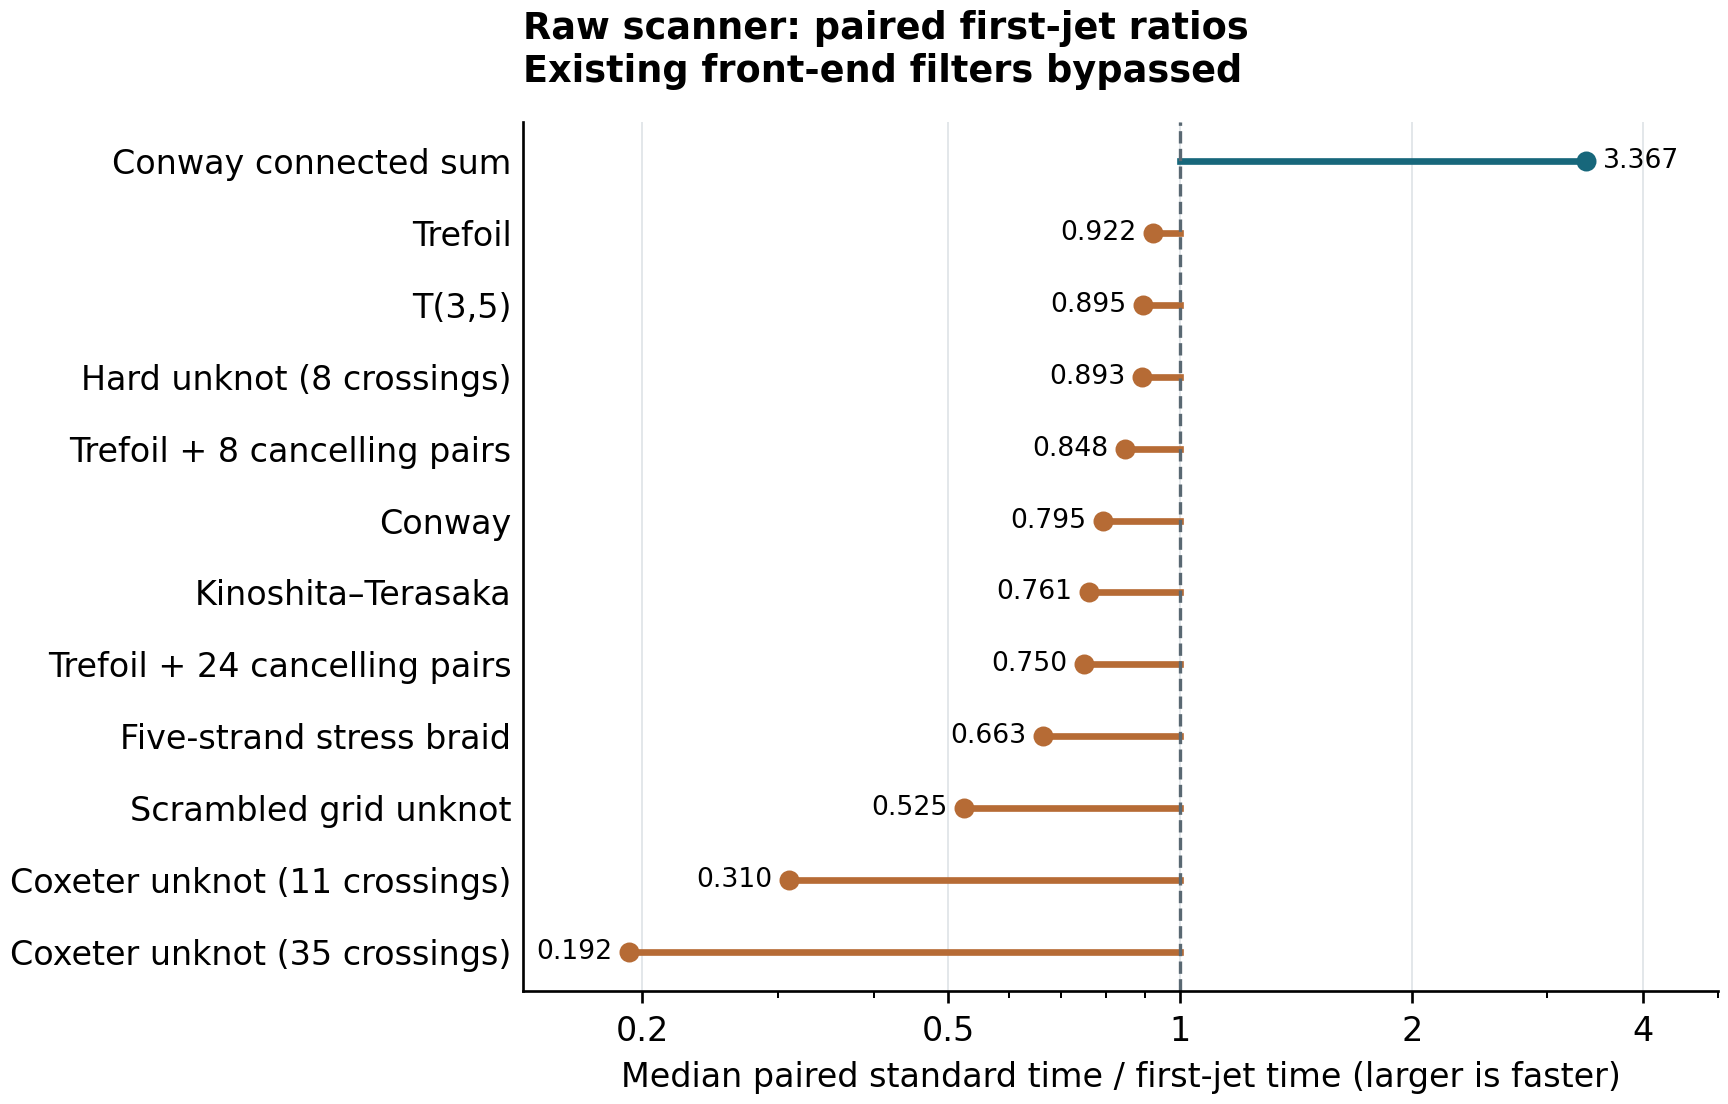
\includegraphics[width=\textwidth]{figures/first_jet_ratios.png}
\caption{All first-jet paired ratios from Table~\ref{tab:jet-timings}.
The dashed line is equal runtime. The early Conway-sum obstruction is
the only improvement in this raw-scanner corpus; replacement cases regress.}
\label{fig:jet-ratios}
\end{figure}

% Derived only from the existing su2_audit.json and su2_benchmark.json.
% No experiments were rerun for this subsection.

\subsection{SU(2) compilation and decision experiments}
\label{subsec:su2-experiments}

The recorded experiments test the exact formula construction and illustrate
the practical degree--variable tradeoff with the exact NLSAT method\cite{JovanovicDeMoura2012,ProgrammingZ3}.  They do not measure the running
time of the theoretical real-decision algorithm.  The complete records are
\path{results/su2_audit.json} and
\path{results/su2_benchmark.json}; the corresponding scripts are
\path{su2_research/audit_su2.py} and
\path{su2_research/benchmark_su2.py}.

\paragraph{Finite correctness audit.}
With seed $20261008$, the audit sampled 48 accepted one-component braid
closures on two to four strands, using words of one to seven letters.
Every third accepted diagram was mirrored.  An independently implemented
reduced $\mathbb F_2$ Khovanov cube classified 39 samples as unknots
and nine as knotted.  Bridge compilation completed 42 of 48 queries:
36 unknot decisions and six knottedness decisions.  Its six timeouts
comprised three samples of each oracle class.  Defining-generator Tietze
elimination followed by compilation completed all 48 queries.  Thus 90 of
96 queries were definitive, with no disagreement among those 90.
The audit identifies its exact backend as Z3 5.1.0.

These are 48 sampled entries, containing 38 distinct stored PD arrays,
and do not constitute 48 distinct knot types or an independent test-set
estimate of general success probability.  The saved PD arrays specify
the actual inputs: the stored source braid words precede the optional
mirroring step.  The seed and script reproduce that step.
For the 36 sampled entries with at most five crossings, comprising 26
distinct PD arrays, exhaustive counts of homomorphisms to $S_3$ agreed
for the Wirtinger, bridge, and simplified presentations.  This checks
concrete relation-order and substitution behavior; agreement for one
finite target group does not establish presentation equivalence in
general.  The Tietze and bridge proofs supply that justification.

The same audit checked the prime-pretzel family at
$m=3,5,7,11,21,51$, hence at $9,15,21,33,63,153$ crossings.
The computed Fox $3$-coloring dimensions were respectively
$3,5,7,11,21,51$, as predicted by
Proposition~\ref{prop:su2-prime-rank-obstruction}.  These finite checks
support the construction and indexing; the proposition's proof supplies
the statement for all odd $m$.

\paragraph{Presentation choice and peak degree.}
The benchmark makes three repetitions per presentation on seven fixed
examples, with a requested solver allowance of $250$ milliseconds.
Table~\ref{tab:su2-recorded-bench} reports representative cases.
Here $k$ is the actual number of real variables after the safe gauge and
meridional trace sharing, and $d_{\rm eq}$ is the maximum degree of an
individual compiled equality before squaring.  The implementation sends
the separate equations to NLSAT in these measurements.  Its sum-of-squares
aggregate is available separately for the constant-atom theoretical bound.

\begin{table}[htbp]
\centering
\small
\begin{tabular}{llrrrrl}
\hline
Input & Presentation & $k$ & $d_{\rm eq}$ & Compile ms & Query ms & Result\\
\hline
Figure-eight & Wirtinger & 10 & 4 & 0.702 & 273.510 & I\\
 & Bridge & 10 & 2 & 0.416 & 270.820 & I\\
 & Tietze & 4 & 10 & 1.716 & 26.103 & K\\
$T(2,9)$ & Wirtinger & 25 & 4 & 1.866 & 283.346 & I\\
 & Bridge & 25 & 2 & 0.972 & 285.034 & I\\
 & Tietze & 4 & 18 & 11.411 & 72.254 & K\\
Coxeter unknot, $n=9$ & Wirtinger & 25 & 4 & 1.519 & 280.035 & I\\
 & Bridge & 2 & 2 & 0.323 & 0.983 & U\\
 & Tietze & 2 & 2 & 0.319 & 1.232 & U\\
\hline
\end{tabular}
\caption{Recorded medians of three repetitions, in milliseconds.  K:
nonabelian representation; U: no nonabelian representation; I:
inconclusive timeout.  All three repetitions in each row had the displayed
status.  The Coxeter example is the closure of
$\sigma_1\cdots\sigma_9\in B_{10}$.  Timeout durations are reported
as censored runs and are not completion times.}
\label{tab:su2-recorded-bench}
\end{table}

On $T(2,9)$, Tietze elimination reduced $k$ from 25 to four while
raising $d_{\rm eq}$ to 18, with aggregate degree bound 36.
Its compilation took longer, but its query completed within the requested
allowance while the other two formulations did not.  This demonstrates
why generator elimination must be assessed together with degree and
support growth.  It gives no finite speedup ratio against a censored run.
Across all 63 benchmark queries, 39 were definitive and 24 inconclusive.

\paragraph{Compressed powers.}
A separate construction-only experiment uses the general presentation
$\langle x_1,x_2\mid x_1^{2^b}\rangle$, represented by $b$ squaring
gates.  It has no knot-group provenance and was not assigned a knot
verdict.  Table~\ref{tab:su2-recorded-powers} shows that the compiler
retained the circuit, producing constant-degree equations without
expanding $2^b$ letters.  The number of stored terms sums the supports
of the individual equations and the nonabelian polynomial; it is not the
support of a fully collected sum-of-squares aggregate.

\begin{table}[htbp]
\centering
\small
\begin{tabular}{rrrrr}
\hline
$b$ & Real variables & Stored terms & $d_{\rm eq}$ & Compile ms\\
\hline
8 & 37 & 97 & 2 & 0.260\\
32 & 133 & 361 & 2 & 0.815\\
128 & 517 & 1417 & 2 & 3.160\\
512 & 2053 & 5641 & 2 & 13.622\\
2048 & 8197 & 22537 & 2 & 54.236\\
\hline
\end{tabular}
\caption{Three-run compiler medians for an already constructed word
circuit.  Expanded word length is $2^b$; aggregate degree bound is four
throughout.  These measurements exclude WordArena construction and make
no claim about solver performance on the resulting formulas.}
\label{tab:su2-recorded-powers}
\end{table}

\paragraph{Interpretation and trust boundary.}
Both scripts enable a trace-zero witness probe before the unrestricted
query. A satisfying assignment to this restricted query is valid for
the original formula; an unsatisfiable or unknown probe is discarded by
this implementation. The known completeness theorem for verified knot
meridians, Theorem~\ref{thm:su2-traceless}, would permit a stronger
knot-specific policy, but these recorded runs do not implement it.
All 15 successful knottedness queries in the audit used this probe.
Their exact algebraic model expressions were retained and checked against
the assertions by Z3 itself.  This remains a trusted-solver computation,
not an independently checked proof certificate.  Neither a trace-zero
failure nor any timeout is accepted as an unknot decision.

The timing allowances are soft: the largest recorded audit call took
$375.926$ milliseconds with a requested $300$-millisecond allowance,
and the largest benchmark query took $288.326$ milliseconds with a
requested $250$-millisecond allowance.  The benchmark's reported query
time includes formula parsing and solver checks, but excludes the Z3
import and subsequent model extraction and validation.  Its compiler
times exclude construction of the input diagram.  The audit's per-call
times cover compilation and the solver wrapper.

The identical repeated compiler controls also show appreciable timing
variation: across 63 pairs, the median first-run/control ratio was 1.234,
with range 0.609--5.565.  Since the control always runs second, this
includes order and warm-up effects.  With three repetitions, fixed case
order, and a small convenience sample, the data justify neither a
statistical speedup claim nor an extrapolated asymptotic exponent.
They document correct completed queries and concrete representation
tradeoffs.  Renegar's theoretical complexity and this optional NLSAT
implementation remain separate statements.


\subsection{Interpreting the response measurements}

Section~\ref{sec:streaming-response} reports the complete all-suffix setup
experiment because its arithmetic and geometry scopes belong together.
At 256 crossings, dense rebuilding takes 3615.101 ms and streaming takes
14.061 ms, a recorded ratio of 257.10; the identical dense control ratio
is 0.906. The new arithmetic theorem, the reduction from 23,789,518 to
928 elimination updates, and the small carried matrices explain the
direction of the gain without depending on an exact wall-clock ratio.

The input family is easy for the recognition front end. The streaming-only
8192-crossing run demonstrates capacity for many evolving suffixes,
not difficulty of those knot types. A future integration experiment
must retain inputs on which the recognizer actually demands many such
responses, and include the setup cost even if an early certificate
ends the scan. The present release therefore makes no default-recognizer
speedup claim from this experiment.

\begin{figure}[htbp]
\centering
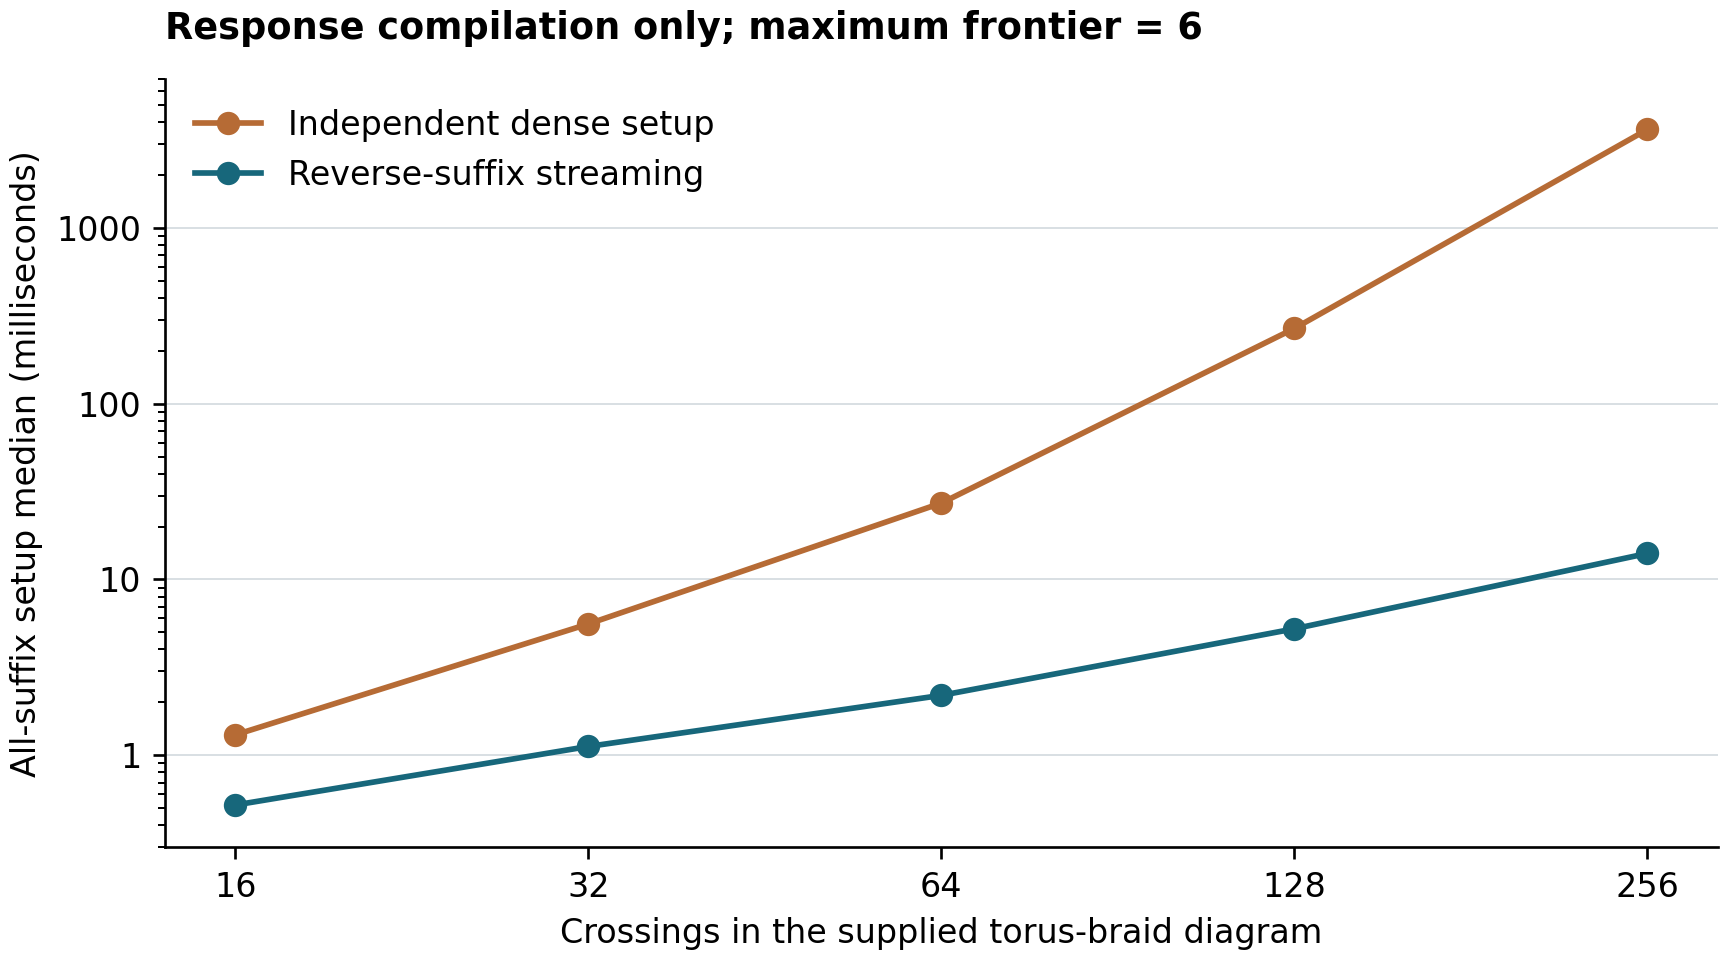
\includegraphics[width=\textwidth]{figures/response_setup.png}
\caption{Recorded all-suffix setup medians at frontier six, with logarithmic
axes. These are easy torus-braid inputs and subroutine timings. The plot
shows the recorded points only; it does not fit an asymptotic exponent.}
\label{fig:response-setup}
\end{figure}

\subsection{What these experiments do not establish}

No finite corpus establishes universal checkpoint bounds, small
presentations, or a success probability on arbitrary knots. No timeout is
counted as an exact answer or as a completed baseline runtime. No
exponent is estimated from the timing table. No synthetic word circuit
is promoted to a knot input without group provenance. The tests and
measurements support implementation claims and identify costs worth
reducing; the asymptotic claims come from the explicit proofs.

\section{Further research questions and a prioritized program}
\label{sec:agenda}

The most useful next step is not simply a larger benchmark. It is to
separate structural hypotheses that might yield a quasi-polynomial theorem
from engineering changes whose value must be established by controlled
whole-query experiments. The questions below specify the desired object,
the proof obligation, and a useful first deliverable.

\subsection{Structural questions bearing directly on the target}

\begin{enumerate}[label=\textbf{Q\arabic*.},leftmargin=3em]
\item \textbf{Which precisely defined residual class admits small
presentation parameters?}
After certified prime decomposition and the maintained structural,
determinant, coloring, and Alexander tests, can the surviving class be
shown to have a constructible circuit cut satisfying
$(r+t)\log(d+2)=O(\log^2 n)$? The filters must be fixed mathematically,
not described as ``all easy cases.'' Begin with prime determinant-one or
Alexander-trivial diagrams and identify whether large ordinary group
rank persists. The displayed dihedral obstructions are removed by cheap
coloring and therefore do not settle this residual question. A counterfamily
would be as useful as a positive theorem, provided it survives the stated
filters and includes a rank or cut lower bound.

\item \textbf{Can one construct small presentations of unknots efficiently?}
Every unknot group has a one-generator presentation, but that existence
does not bound the cost of finding it from a difficult diagram. Seek a
family of verified Tietze or geometric transformations with bounded move
count, grammar growth, and compressed verification cost on unknots.
Separate unknotted-input guarantees from the separate task of rejecting
knotted inputs. A proof that a local search never stalls requires a
global completeness argument, and any temporary word expansion must be
charged in its actual representation.

\item \textbf{Can the decision problem use smaller data than the whole group?}
The rank obstructions rule out a universal small presentation of the
entire group, not a small certificate tailored to triviality. One could
seek verified decompositions, representation-preserving quotients, or
local extension problems whose conjunction detects the unknot. A proposed
quotient must preserve the direction needed: a nonabelian image of a
quotient certifies knottedness, whereas failure to find one generally
does not certify the unknot. A complete reduction needs both directions
and a bound on the size and number of subproblems.

\item \textbf{Can checkpoint gaps and frontier widths be controlled together?}
Construct crossing orders or certified splicing moves with
$g+w=O(\log^2 n)$ on a meaningful class of hard residual diagrams.
The gap must include the crossing that triggers a replacement and the
last segment; the width must be the actual temporary frontier. Study
whether alternating reductions, arborescent decompositions, or controlled
tangle sums give such orders after the already easy cases are removed.
A bound only on final survivor count leaves the intermediate cost unresolved.

\item \textbf{Can geometric hierarchy certificates supply the missing size theorem?}
Translate the hierarchy parameters in \cite{Lackenby2026Hierarchies} into
explicit data structures and verified transitions. Bound hierarchy length,
surface and pattern complexity, compressed cutting cost, and the bit
length of every update. The displayed iteration bound $L(g+1)^L$ is
only one term in that analysis. A practical starting point is a small
certificate checker for one cutting or simplification step, with
independent topology reconstruction and a precise input-size theorem.

\item \textbf{What exactly is established by the recent bridge-minimization claim?}
Independently audit \cite{Musick2026}, including conversion from arbitrary
input diagrams, completeness of the allowed moves, the application of
Otal's theorem to the unknot case, and polynomial
bounds for their actual encoded
execution. Record any lemma that requires an additional hypothesis and
distinguish implementation tests from proof of that lemma. The present
report's results do not assume the claim; resolving its status would
materially change the broader research landscape.
\end{enumerate}

\subsection{Algebraic compilation and exact certificates}

\begin{enumerate}[label=\textbf{Q\arabic*.},leftmargin=3em,start=7]
\item \textbf{How hard is the best word-circuit cut?}
Study the optimization problem
$\min_C(r+|C|)\log(d_C+2)$ on a word DAG. A first target is an exact
dynamic program for trees, followed by a proved approximation or a
parameterized algorithm for shared DAGs. Repeated subwords make local
greedy cuts potentially suboptimal. Formal degree, actual monomial
support, coefficient height, and compiler work can be tracked separately;
an empirical support heuristic should not be substituted into the
worst-case theorem without a bound.

\item \textbf{Can quaternion-specific identities improve the degree bound?}
Repeated powers of a unit quaternion satisfy a quadratic recurrence, so
Chebyshev-type representations may compress certain relators further.
Any use of these identities must preserve all unit-quaternion solutions,
including central generators, and count newly introduced scalar or
quaternion variables. Determine whether power-heavy knot presentations
admit smaller cuts than generic straight-line words. Avoid confusing a
short recurrence with a constant-cost real formula.

\item \textbf{Can exact representation witnesses be checked independently?}
The current optional solver records algebraic models and checks its
assertions through the same exact engine. A stronger SAT artifact would
give isolating intervals, defining polynomials, and independently verified
sign tests for every equation and the noncommutativity inequality. For
UNSAT, specify a checkable real-algebraic proof format or a verified
decision backend. Establish verifier complexity in the certificate's
actual bit size; a compact approximate numerical model alone is insufficient.

\item \textbf{How should the known traceless-meridian theorem be used?}
Kronheimer--Mrowka already prove complete detection with a meridian
sent to $i$ \cite[Corollary~7.17]{KM2010Excision}; this is not an open
trace-existence question. Implement and independently validate
Corollary~\ref{cor:su2-fixed-meridian}, carrying explicit meridional
provenance through generator changes. Compare its smaller complete formula
with the current one-sided witness probe on the same residual corpus.
A separate mathematical question concerns other prescribed trace values
or trace schedules that improve real-algebraic decomposition. Such a
restriction requires its own theorem, and generic nonmeridional
generators must retain the unrestricted query.

\item \textbf{Can presentation provenance remain compressed across every move?}
The repository already independently replays several compressed group
certificates. Connect that verifier to the new circuit compiler so arbitrary
generator changes switch correctly from the meridional inequality to the
general commutator condition. Bound grammar size and assertion growth
through long traces, not just individual word operations. The first
deliverable should be a shared, versioned presentation object carrying
origin, generator meanings, and exactly the current relators.
\end{enumerate}

\subsection{Earlier homological decisions and reusable geometry}

\begin{enumerate}[label=\textbf{Q\arabic*.},leftmargin=3em,start=12]
\item \textbf{Can the flat-origin constraint remove the second rank safely?}
For genuine minimal same-matching components, $\kappa=t$. Determine how
to maintain a cheap connection or provenance certificate across scalar
cancellation, direct-summand extraction, and total-rank replacements.
The last operation need not preserve genuine cube origin. A theorem
covering exactly the executed scanner would permit using one rank where
two are currently computed. Merely observing $t=\kappa$ in a corpus is
not sufficient to install that shortcut.

\item \textbf{What constraints survive in higher jets or mixed matchings?}
Lift the identity $\partial Q=\Gamma Q+Q\Gamma$ beyond scalar residue.
Can it restrict higher-dot coefficients, transferred operations, or the
shape of mixed-matching minimal blocks enough to bound multiplicities?
The objective is a genuine realizability constraint on tangle-derived
complexes. Arbitrary polynomial complexes over the dot algebra may be
too broad to support the desired theorem, as the synthetic odd intervals
already demonstrate.

\item \textbf{Can eligible components be maintained incrementally?}
Current graph traversal and binary ranks can cost more than the scalar
cancellations they avoid. Develop a dynamic index that certifies a
whole one-matching direct summand and updates its scalar matrix after one
crossing. It must detect all external attachments and survive transactional
interruption. Evaluate saved cobordism compositions against the cost of
component maintenance; the present easy replacement families regress.

\item \textbf{When should a scan precompute suffix responses?}
Develop an adaptive policy that chooses independent setup, checkpoint
responses, or full reverse compilation based on a proved cost estimate
and observed demand. Aim for a competitive bound relative to the better
strategy, including source geometry and abandoned work. A forward scanner
may terminate before most precomputed suffixes are queried. The large
all-stage timing ratios therefore cannot directly choose a default policy.

\item \textbf{Can a separator tree support local response updates?}
Replace the linear order by a decomposition tree while retaining radical
couplings and exact grounding. Prove a boundary contract that permits
subtree changes without identifying eliminated interior vertices. Determine
which snapshots and Euler summaries can be shared across primes or nearby
orders despite exceptional pivot profiles. The established low-treewidth
linear-algebra literature provides a starting point, not a substitute for
the topology-specific gluing proof \cite{furer-hoppen-trevisan}.
\end{enumerate}

\subsection{Evidence, dispatch, and a concrete sequence of deliverables}

\begin{enumerate}[label=\textbf{Q\arabic*.},leftmargin=3em,start=17]
\item \textbf{Which residual corpus measures the intended improvement?}
Assemble difficult unknots and knots that survive the exact existing
front ends, with full PD provenance, mirrors, several orders, and
duplicate detection. Include determinant-one and Alexander-trivial knots,
inflated unknots, and examples with substantial repeated suffix interior
work. A test label should come from an independent certificate or complete
oracle. Synthetic word circuits remain useful for capacity tests but
must be reported separately from knot-recognition instances.

\item \textbf{Which optional method improves complete queries reliably?}
Run paired, shuffled whole-recognizer experiments with identical controls,
fixed source hashes, explicit warmup rules, and all outcomes retained.
Report CPU and wall time scopes, object and coefficient peaks, solver
startup, model validation, and censored runs. Promotion to a default
should require a reproducible benefit on the target residual corpus
without a correctness or deadline regression. A small local improvement
does not justify hiding a larger all-stage setup cost.
\end{enumerate}

The proposed order is concrete. First, finish the residual corpus and
attach independently checked presentation provenance to the representation
compiler. Next, reduce first-jet traversal overhead and prototype an
adaptive response consumer, retaining the present backends as controls.
In parallel, pursue either a circuit-cut theorem for a precisely filtered
class or a geometric bound on checkpoint gaps and frontier width. A
successful structural theorem would immediately plug into
Corollary~\ref{cor:regimes}; until then, the optional implementations and
recorded negative results provide a disciplined experimental platform.

\appendix
\section{Reproduction and integration notes}
\label{sec:reproduce}

\subsection{Pinned source and package contents}

The baseline is the public repository commit \basecommit. The companion
archive includes this article's complete \LaTeX{} source and bibliography,
the compiled PDF, an integration patch, a reviewable tree of changed and
new repository files, and a runnable source snapshot with the independent
test-oracle files needed by the existing suite. Machine-readable manifests
record source provenance and SHA-256 digests. Temporary bytecode caches,
compiler intermediates, and failed retrieval artifacts are excluded.

The new implementation files are
\path{fastunknot/su2.py}, \path{fastunknot/first_jet.py},
\path{fastunknot/first_jet_scan.py}, and
\path{fastunknot/streaming_response.py}. Each has focused tests.
Raw measurements and inputs live in \path{fast/results/}; replay
scripts are grouped by experiment. The default recognizer does not
automatically select these new research backends.

One existing file, \path{fastunknot/normal_surface.py}, receives an
inherited correction from the preceding research continuation. Repeated
\texttt{communicate(None)} calls after a timeout can lose an incompletely
sent input payload on the supported Python subprocess path. The corrected
worker performs exactly one \texttt{communicate(payload)} in a thread,
polls its completion under the cooperative deadline, and kills, reaps,
and joins on interruption. This resolves the existing
\texttt{test\_communication\_retains\_input\_across\_polls} regression.
It is an integration fix with prior provenance, not a new mathematical
or recognition-performance result of this article.

\subsection{Build and test commands}

The article uses standard \LaTeX{} packages; no external network source
is needed to compile it. From the article directory:
\par\noindent\begin{minipage}{\linewidth}
\begin{lstlisting}
latexmk -pdf -interaction=nonstopmode -halt-on-error \
  unknot_presentations_and_early_certificates.tex
\end{lstlisting}
\end{minipage}\par
An already generated bibliography is included for installations that
prefer a plain \texttt{pdflatex} build; a complete refresh uses BibTeX
through \texttt{latexmk}. The archived PDF is rendered and visually
checked after compilation.

From the bundled or patched \path{Topology/UnknotRecognition/fast}
directory:
\par\noindent\begin{minipage}{\linewidth}
\begin{lstlisting}
python3 -m unittest discover -s tests -q
python3 first_jet_research/audit.py --fast-root . \
  --output results/first_jet_discovery_local.json
python3 benchmark_first_jet.py \
  --output results/first_jet_benchmark_local.json
python3 response_research/audit_streaming_response.py \
  --output results/streaming_response_audit_local.json
python3 response_research/benchmark_streaming_response.py \
  --output results/streaming_response_local.json \
  --sizes 16 32 64 128 --rounds 7 --large-stream 2048
python3 response_research/benchmark_streaming_response.py \
  --output results/streaming_response_large_local.json \
  --sizes 256 --rounds 3 --large-stream 8192
python3 su2_research/audit_su2.py \
  --output results/su2_audit_local.json
python3 su2_research/benchmark_su2.py \
  --output results/su2_benchmark_local.json
\end{lstlisting}
\end{minipage}\par
The detailed README gives the accepted output-path and size flags of
each script. The recorded optional real solver is
\path{z3-solver==5.1.0.0}, reporting core version 5.1.0. The symbolic
compiler, exact rational-witness tests, finite-group checks, first-jet
code, and response code do not need that dependency. Solver-dependent
tests skip when it is absent.

The complete integrated suite depends on the bundled independent
reference modules from reports 24, 26, and 28. They are unchanged copies
of pinned repository files, not a second implementation of the new
incremental state inside its oracle. Existing optional Regina tests
remain conditional on that external dependency.

\subsection{Example interfaces}

The following generic query has no knot verdict attached:
\par\noindent\begin{minipage}{\linewidth}
\begin{lstlisting}[language=Python]
from fastunknot.su2 import compile_presentation, solve_formula

# The trefoil presentation aba = bab, supplied here only as a group.
formula = compile_presentation(
    [1, 2], [(1, 2, 1, -2, -1, -2)], chunk_size=3
)
print(formula.summary())
print(solve_formula(formula, seconds=1.0))
\end{lstlisting}
\end{minipage}\par
Use the validated diagram constructor to obtain a knot decision:
\par\noindent\begin{minipage}{\linewidth}
\begin{lstlisting}[language=Python]
from fastunknot.diagram import Diagram
from fastunknot.su2 import su2_decide

d = Diagram.from_braid(3, [1, -2, 1, -2])
answer = su2_decide(d, presentation="tietze", seconds=1.0,
                    trace_zero_probe=True)
print(answer["status"])
\end{lstlisting}
\end{minipage}\par
The trace-zero flag enables a one-sided witness probe only. This interface
still queries the full formula after a failed restricted probe; it does
not exploit the stronger complete specialization in
Corollary~\ref{cor:su2-fixed-meridian}. Export an
exact SMT-LIB input with the standalone CLI's \texttt{--smt2} option.

The rank-only scanner accepts validated PD data and an optional supplied
order:
\par\noindent\begin{minipage}{\linewidth}
\begin{lstlisting}[language=Python]
from fastunknot.first_jet_scan import first_jet_khovanov_decide

answer = first_jet_khovanov_decide(
    d.pd, seconds=2.0, max_objects=50000,
    first_jet_max_work=1000000
)
print(answer["status"], answer["first_jet_stats"])
\end{lstlisting}
\end{minipage}\par
Its global scan limit is an exception in this raw API, consistent with
the maintained raw scanner contract. A caller must handle that as
unresolved. It must not expose replacement degree counts as the original
graded homology.

Finally, the response compiler takes a crossing order and a prime:
\par\noindent\begin{minipage}{\linewidth}
\begin{lstlisting}[language=Python]
from fastunknot.streaming_response import compile_suffix_responses

responses = compile_suffix_responses(
    d.pd, order=list(range(d.crossings)), prime=101,
    max_boundary=100, max_stored_elements=1000000
)
# Query a stage only with a checked matching on that stage's boundary.
\end{lstlisting}
\end{minipage}\par
The storage allowance counts retained matrix entries; it is not a hard
process-memory cap. Source data and a current temporary matrix have the
additional costs proved in the response theorem.

\subsection{Reproducibility and trust limitations}

All mathematical proofs are presented for review rather than described
as formally verified. Independent implementations and cross-checks reduce
implementation risk, but finite tests do not replace those proofs. The
optional real solver is an explicit trusted backend. SAT models are
retained as exact algebraic expressions and evaluated by that same
backend, while UNSAT is its exact decision result; no independent
UNSAT proof checker is bundled.

The source snapshot is a convenience for reproduction, not a substitute
for reviewing the small integration patch against the pinned repository.
The archive is prepared for later repository integration. It does not
represent a pushed commit or a published change to ProveIt.

\bibliographystyle{plainnat}
\bibliography{references}
\end{document}
